% Options for packages loaded elsewhere
\PassOptionsToPackage{unicode}{hyperref}
\PassOptionsToPackage{hyphens}{url}
%
\documentclass[
]{article}
\usepackage{amsmath,amssymb}
\usepackage{iftex}
\ifPDFTeX
  \usepackage[T1]{fontenc}
  \usepackage[utf8]{inputenc}
  \usepackage{textcomp} % provide euro and other symbols
\else % if luatex or xetex
  \usepackage{unicode-math} % this also loads fontspec
  \defaultfontfeatures{Scale=MatchLowercase}
  \defaultfontfeatures[\rmfamily]{Ligatures=TeX,Scale=1}
\fi
\usepackage{lmodern}
\ifPDFTeX\else
  % xetex/luatex font selection
\fi
% Use upquote if available, for straight quotes in verbatim environments
\IfFileExists{upquote.sty}{\usepackage{upquote}}{}
\IfFileExists{microtype.sty}{% use microtype if available
  \usepackage[]{microtype}
  \UseMicrotypeSet[protrusion]{basicmath} % disable protrusion for tt fonts
}{}
\makeatletter
\@ifundefined{KOMAClassName}{% if non-KOMA class
  \IfFileExists{parskip.sty}{%
    \usepackage{parskip}
  }{% else
    \setlength{\parindent}{0pt}
    \setlength{\parskip}{6pt plus 2pt minus 1pt}}
}{% if KOMA class
  \KOMAoptions{parskip=half}}
\makeatother
\usepackage{xcolor}
\usepackage[margin=1in]{geometry}
\usepackage{color}
\usepackage{fancyvrb}
\newcommand{\VerbBar}{|}
\newcommand{\VERB}{\Verb[commandchars=\\\{\}]}
\DefineVerbatimEnvironment{Highlighting}{Verbatim}{commandchars=\\\{\}}
% Add ',fontsize=\small' for more characters per line
\usepackage{framed}
\definecolor{shadecolor}{RGB}{248,248,248}
\newenvironment{Shaded}{\begin{snugshade}}{\end{snugshade}}
\newcommand{\AlertTok}[1]{\textcolor[rgb]{0.94,0.16,0.16}{#1}}
\newcommand{\AnnotationTok}[1]{\textcolor[rgb]{0.56,0.35,0.01}{\textbf{\textit{#1}}}}
\newcommand{\AttributeTok}[1]{\textcolor[rgb]{0.13,0.29,0.53}{#1}}
\newcommand{\BaseNTok}[1]{\textcolor[rgb]{0.00,0.00,0.81}{#1}}
\newcommand{\BuiltInTok}[1]{#1}
\newcommand{\CharTok}[1]{\textcolor[rgb]{0.31,0.60,0.02}{#1}}
\newcommand{\CommentTok}[1]{\textcolor[rgb]{0.56,0.35,0.01}{\textit{#1}}}
\newcommand{\CommentVarTok}[1]{\textcolor[rgb]{0.56,0.35,0.01}{\textbf{\textit{#1}}}}
\newcommand{\ConstantTok}[1]{\textcolor[rgb]{0.56,0.35,0.01}{#1}}
\newcommand{\ControlFlowTok}[1]{\textcolor[rgb]{0.13,0.29,0.53}{\textbf{#1}}}
\newcommand{\DataTypeTok}[1]{\textcolor[rgb]{0.13,0.29,0.53}{#1}}
\newcommand{\DecValTok}[1]{\textcolor[rgb]{0.00,0.00,0.81}{#1}}
\newcommand{\DocumentationTok}[1]{\textcolor[rgb]{0.56,0.35,0.01}{\textbf{\textit{#1}}}}
\newcommand{\ErrorTok}[1]{\textcolor[rgb]{0.64,0.00,0.00}{\textbf{#1}}}
\newcommand{\ExtensionTok}[1]{#1}
\newcommand{\FloatTok}[1]{\textcolor[rgb]{0.00,0.00,0.81}{#1}}
\newcommand{\FunctionTok}[1]{\textcolor[rgb]{0.13,0.29,0.53}{\textbf{#1}}}
\newcommand{\ImportTok}[1]{#1}
\newcommand{\InformationTok}[1]{\textcolor[rgb]{0.56,0.35,0.01}{\textbf{\textit{#1}}}}
\newcommand{\KeywordTok}[1]{\textcolor[rgb]{0.13,0.29,0.53}{\textbf{#1}}}
\newcommand{\NormalTok}[1]{#1}
\newcommand{\OperatorTok}[1]{\textcolor[rgb]{0.81,0.36,0.00}{\textbf{#1}}}
\newcommand{\OtherTok}[1]{\textcolor[rgb]{0.56,0.35,0.01}{#1}}
\newcommand{\PreprocessorTok}[1]{\textcolor[rgb]{0.56,0.35,0.01}{\textit{#1}}}
\newcommand{\RegionMarkerTok}[1]{#1}
\newcommand{\SpecialCharTok}[1]{\textcolor[rgb]{0.81,0.36,0.00}{\textbf{#1}}}
\newcommand{\SpecialStringTok}[1]{\textcolor[rgb]{0.31,0.60,0.02}{#1}}
\newcommand{\StringTok}[1]{\textcolor[rgb]{0.31,0.60,0.02}{#1}}
\newcommand{\VariableTok}[1]{\textcolor[rgb]{0.00,0.00,0.00}{#1}}
\newcommand{\VerbatimStringTok}[1]{\textcolor[rgb]{0.31,0.60,0.02}{#1}}
\newcommand{\WarningTok}[1]{\textcolor[rgb]{0.56,0.35,0.01}{\textbf{\textit{#1}}}}
\usepackage{longtable,booktabs,array}
\usepackage{calc} % for calculating minipage widths
% Correct order of tables after \paragraph or \subparagraph
\usepackage{etoolbox}
\makeatletter
\patchcmd\longtable{\par}{\if@noskipsec\mbox{}\fi\par}{}{}
\makeatother
% Allow footnotes in longtable head/foot
\IfFileExists{footnotehyper.sty}{\usepackage{footnotehyper}}{\usepackage{footnote}}
\makesavenoteenv{longtable}
\usepackage{graphicx}
\makeatletter
\newsavebox\pandoc@box
\newcommand*\pandocbounded[1]{% scales image to fit in text height/width
  \sbox\pandoc@box{#1}%
  \Gscale@div\@tempa{\textheight}{\dimexpr\ht\pandoc@box+\dp\pandoc@box\relax}%
  \Gscale@div\@tempb{\linewidth}{\wd\pandoc@box}%
  \ifdim\@tempb\p@<\@tempa\p@\let\@tempa\@tempb\fi% select the smaller of both
  \ifdim\@tempa\p@<\p@\scalebox{\@tempa}{\usebox\pandoc@box}%
  \else\usebox{\pandoc@box}%
  \fi%
}
% Set default figure placement to htbp
\def\fps@figure{htbp}
\makeatother
\setlength{\emergencystretch}{3em} % prevent overfull lines
\providecommand{\tightlist}{%
  \setlength{\itemsep}{0pt}\setlength{\parskip}{0pt}}
\setcounter{secnumdepth}{-\maxdimen} % remove section numbering
\usepackage{bookmark}
\IfFileExists{xurl.sty}{\usepackage{xurl}}{} % add URL line breaks if available
\urlstyle{same}
\hypersetup{
  pdftitle={Appendix. A: Summary of R code used in statistical analyses and visualisation. R version 4.5.1.},
  pdfauthor={Mako Shibata},
  hidelinks,
  pdfcreator={LaTeX via pandoc}}

\title{Appendix. A: Summary of R code used in statistical analyses and
visualisation. R version 4.5.1.}
\author{Mako Shibata}
\date{}

\begin{document}
\maketitle

\section{Preamble}\label{preamble}

\subsubsection{Packages}\label{packages}

\begin{Shaded}
\begin{Highlighting}[]
\FunctionTok{library}\NormalTok{(tidyr) }\CommentTok{\#formatting}
\FunctionTok{library}\NormalTok{(dplyr) }\CommentTok{\#manipulation }
\FunctionTok{library}\NormalTok{(ggplot2) }\CommentTok{\#visualisation}
\FunctionTok{library}\NormalTok{(readr) }\CommentTok{\#manipulation}
\FunctionTok{library}\NormalTok{(ggpubr) }\CommentTok{\#visualisation}
\FunctionTok{library}\NormalTok{(knitr) }\CommentTok{\#visualisation}
\FunctionTok{library}\NormalTok{(stats) }\CommentTok{\#power analysis}
\FunctionTok{library}\NormalTok{(pander) }\CommentTok{\#visualisation}
\FunctionTok{library}\NormalTok{(broom) }\CommentTok{\#visualisation}
\end{Highlighting}
\end{Shaded}

\subsubsection{Load Data}\label{load-data}

\begin{Shaded}
\begin{Highlighting}[]
\CommentTok{\# set working directory }
\FunctionTok{setwd}\NormalTok{(}\StringTok{"/Users/Owner/Library/CloudStorage/OneDrive{-}UniversityofEdinburgh/\#00\_EM/Project\_Soil Microclimate/EM\_SoilMicroclimate"}\NormalTok{)}

\CommentTok{\# load raw data}
\NormalTok{soil }\OtherTok{\textless{}{-}} \FunctionTok{read.csv}\NormalTok{(}\StringTok{"RAW\_ALL\_soil\_microclimate.csv"}\NormalTok{)}

\CommentTok{\# combine tree species entry into one column}
\CommentTok{\# remove unnecessary columns}
\NormalTok{soil }\OtherTok{\textless{}{-}}\NormalTok{ soil }\SpecialCharTok{\%\textgreater{}\%}
  \FunctionTok{mutate}\NormalTok{(}\AttributeTok{Tree.species =} \FunctionTok{if\_else}\NormalTok{(}
\NormalTok{    Tree.species }\SpecialCharTok{==} \StringTok{"other"}\NormalTok{, }
\NormalTok{    Other..specify....Tree.species, }
\NormalTok{    Tree.species)) }\SpecialCharTok{\%\textgreater{}\%}
  \FunctionTok{select}\NormalTok{(}\SpecialCharTok{{-}}\NormalTok{Other..specify....Tree.species, }
         \SpecialCharTok{{-}}\NormalTok{Mixed.Other..specify....Ground.Cover.Types, }
         \SpecialCharTok{{-}}\NormalTok{Ground.Cover.Types)}

\CommentTok{\# create a long format data, gathered by Distance (0.5 and 7.0 m)}
\NormalTok{soil0}\FloatTok{.5} \OtherTok{\textless{}{-}}\NormalTok{ soil }\SpecialCharTok{\%\textgreater{}\%} 
  \FunctionTok{select}\NormalTok{(}\AttributeTok{Date =}\NormalTok{ Date...Time, }
         \AttributeTok{TreeID =}\NormalTok{ Tree.Plot.ID.., }
         \AttributeTok{Species =}\NormalTok{ Tree.species, }
         \AttributeTok{DBH\_cm =}\NormalTok{ DBH..cm., }
         \AttributeTok{Cardinal =}\NormalTok{ Cardinal.Direction, }
         \AttributeTok{Depth\_cm =}\NormalTok{ Soil.organic.layer.depth..cm., }
         \AttributeTok{Moisture\_vv =}\NormalTok{ Soil.moisture....V.V., }
         \AttributeTok{Distance =}\NormalTok{ Distance.from.tree.trunk..m., }
         \AttributeTok{Notes =}\NormalTok{ Notes...Comments, }
         \AttributeTok{x =}\NormalTok{ x, }
         \AttributeTok{y =}\NormalTok{ y}
\NormalTok{         )}

\NormalTok{soil7}\FloatTok{.0} \OtherTok{\textless{}{-}}\NormalTok{ soil }\SpecialCharTok{\%\textgreater{}\%} 
  \FunctionTok{select}\NormalTok{(}\AttributeTok{Date =}\NormalTok{ Date...Time, }
         \AttributeTok{TreeID =}\NormalTok{ Tree.Plot.ID.., }
         \AttributeTok{Species =}\NormalTok{ Tree.species, }
         \AttributeTok{DBH\_cm =}\NormalTok{ DBH..cm., }
         \AttributeTok{Cardinal =}\NormalTok{ Cardinal.Direction, }
         \AttributeTok{Depth\_cm =}\NormalTok{ Soil.organic.layer.depth..cm..}\DecValTok{1}\NormalTok{, }
         \AttributeTok{Moisture\_vv =}\NormalTok{ Soil.moisture....V.V..}\DecValTok{1}\NormalTok{, }
         \AttributeTok{Distance =}\NormalTok{ Distance.from.tree.trunk..m..}\DecValTok{1}\NormalTok{, }
         \AttributeTok{Notes =}\NormalTok{ Notes...Comments, }
         \AttributeTok{x =}\NormalTok{ x, }
         \AttributeTok{y =}\NormalTok{ y}
\NormalTok{  )}

\NormalTok{soil\_all }\OtherTok{\textless{}{-}} \FunctionTok{bind\_rows}\NormalTok{(soil0}\FloatTok{.5}\NormalTok{, soil7}\FloatTok{.0}\NormalTok{) }\SpecialCharTok{\%\textgreater{}\%}
  \FunctionTok{arrange}\NormalTok{(TreeID, Distance) }\SpecialCharTok{\%\textgreater{}\%}
  \FunctionTok{mutate}\NormalTok{(}\AttributeTok{running\_order =} \FunctionTok{row\_number}\NormalTok{()) }\SpecialCharTok{\%\textgreater{}\%}
  \FunctionTok{relocate}\NormalTok{(running\_order, }\AttributeTok{.before =}\NormalTok{ TreeID) }\SpecialCharTok{\%\textgreater{}\%} 
  \FunctionTok{select}\NormalTok{(}\SpecialCharTok{{-}}\NormalTok{Notes)}

\CommentTok{\# set distance as a factor }
\NormalTok{soil\_all}\SpecialCharTok{$}\NormalTok{Distance }\OtherTok{\textless{}{-}} \FunctionTok{as.factor}\NormalTok{(soil\_all}\SpecialCharTok{$}\NormalTok{Distance)}
\CommentTok{\# omit N/A rows }
\NormalTok{soil\_all }\OtherTok{\textless{}{-}} \FunctionTok{na.omit}\NormalTok{(soil\_all)}
\end{Highlighting}
\end{Shaded}

\subsubsection{Clean data}\label{clean-data}

The following procedure corrects the species mis-entry (English Oak to
Silver Birch), adds a column of Genus and management types for
group-specific analyses, and creates a new data frame with no Scots Pine
data. Scots Pine is removed due to its sample size being 1.

\begin{Shaded}
\begin{Highlighting}[]
\CommentTok{\# replace oak with birch, set genus name in a new column. }
\NormalTok{soil\_all }\OtherTok{\textless{}{-}}\NormalTok{ soil\_all }\SpecialCharTok{\%\textgreater{}\%} 
  \FunctionTok{mutate}\NormalTok{(}\AttributeTok{Species =} \FunctionTok{recode}\NormalTok{(Species,}
                          \StringTok{"English Oak (Quercus robur)"} \OtherTok{=} \StringTok{"Silver Birch (Betula pendula)"}\NormalTok{)) }\SpecialCharTok{\%\textgreater{}\%}
  \FunctionTok{mutate}\NormalTok{(}\AttributeTok{Genus =} \FunctionTok{case\_when}\NormalTok{(}
\NormalTok{    Species }\SpecialCharTok{==} \StringTok{"Alder"} \SpecialCharTok{\textasciitilde{}} \StringTok{"Alnus"}\NormalTok{, }
\NormalTok{    Species }\SpecialCharTok{==} \StringTok{"Silver Birch (Betula pendula)"} \SpecialCharTok{\textasciitilde{}} \StringTok{"Betula"}\NormalTok{, }
\NormalTok{    Species }\SpecialCharTok{==} \StringTok{"Downy Birch (Betula pubescens)"} \SpecialCharTok{\textasciitilde{}} \StringTok{"Betula"}\NormalTok{,}
\NormalTok{    Species }\SpecialCharTok{==} \StringTok{"Scots pine (Pinus sylvestris)"} \SpecialCharTok{\textasciitilde{}} \StringTok{"Pinus"}\NormalTok{,}
\NormalTok{    Species }\SpecialCharTok{==} \StringTok{"Rowan (Sorbus aucuparia)"} \SpecialCharTok{\textasciitilde{}} \StringTok{"Sorbus"}
\NormalTok{  ))  }\SpecialCharTok{\%\textgreater{}\%}
  \FunctionTok{relocate}\NormalTok{(Genus, }\AttributeTok{.before =}\NormalTok{ Species)}

\CommentTok{\# create a management type column using TreeID that falls within a specific management regime}
\NormalTok{soil\_all}\OtherTok{\textless{}{-}}\NormalTok{ soil\_all }\SpecialCharTok{\%\textgreater{}\%} 
  \FunctionTok{mutate}\NormalTok{(soil\_all, }\AttributeTok{Management =} \FunctionTok{case\_when}\NormalTok{(}
\NormalTok{    TreeID }\SpecialCharTok{\%in\%} \FunctionTok{c}\NormalTok{(}\DecValTok{1}\NormalTok{, }\DecValTok{2}\NormalTok{, }\DecValTok{3}\NormalTok{, }\DecValTok{4}\NormalTok{, }\DecValTok{5}\NormalTok{, }\DecValTok{6}\NormalTok{, }\DecValTok{7}\NormalTok{, }\DecValTok{21}\NormalTok{, }\DecValTok{22}\NormalTok{, }\DecValTok{23}\NormalTok{, }\DecValTok{24}\NormalTok{, }\DecValTok{25}\NormalTok{) }\SpecialCharTok{\textasciitilde{}} \StringTok{"No mound"}\NormalTok{, }
    \ConstantTok{TRUE} \SpecialCharTok{\textasciitilde{}} \StringTok{"mound"}\NormalTok{)) }\SpecialCharTok{\%\textgreater{}\%}
  \FunctionTok{relocate}\NormalTok{(Management, }\AttributeTok{.after =}\NormalTok{ Species)}

\CommentTok{\# save cleaned data including pine }
\FunctionTok{write.csv}\NormalTok{(soil\_all, }\StringTok{"soil\_all.csv"}\NormalTok{)}

\CommentTok{\# remove pine}
\NormalTok{soil\_all\_nonpine }\OtherTok{\textless{}{-}}\NormalTok{ soil\_all }\SpecialCharTok{\%\textgreater{}\%} 
  \FunctionTok{filter}\NormalTok{(Genus }\SpecialCharTok{!=} \StringTok{"Pinus"}\NormalTok{) }

\CommentTok{\# save cleaned data excluding pine }
\FunctionTok{write.csv}\NormalTok{(soil\_all\_nonpine, }\StringTok{"soil\_all\_nonpine.csv"}\NormalTok{)}
\end{Highlighting}
\end{Shaded}

\section{DBH (cm) and Age}\label{dbh-cm-and-age}

The following codes calculated mean, standard deviation, max, and
minimum of DBH (cm) for total species and all genus groups. DBH is
converted to age by applying a growth factor of 2.5 cm/year (Mitchell,
1974).

\begin{Shaded}
\begin{Highlighting}[]
\CommentTok{\# read soil\_all\_pine as soil}
\NormalTok{soil }\OtherTok{\textless{}{-}}\NormalTok{ soil\_all\_nonpine}
\CommentTok{\# get average DBH (cm) +{-} std for the following groups: total, alder, birch, sorbus}
\NormalTok{DBH\_mean }\OtherTok{\textless{}{-}} \FunctionTok{c}\NormalTok{(}\FunctionTok{mean}\NormalTok{(soil}\SpecialCharTok{$}\NormalTok{DBH\_cm),}
              \FunctionTok{mean}\NormalTok{(soil}\SpecialCharTok{$}\NormalTok{DBH\_cm[soil}\SpecialCharTok{$}\NormalTok{Genus }\SpecialCharTok{==} \StringTok{"Alnus"}\NormalTok{]),}
              \FunctionTok{mean}\NormalTok{(soil}\SpecialCharTok{$}\NormalTok{DBH\_cm[soil}\SpecialCharTok{$}\NormalTok{Genus }\SpecialCharTok{==} \StringTok{"Betula"}\NormalTok{]),}
              \FunctionTok{mean}\NormalTok{(soil}\SpecialCharTok{$}\NormalTok{DBH\_cm[soil}\SpecialCharTok{$}\NormalTok{Genus }\SpecialCharTok{==} \StringTok{"Sorbus"}\NormalTok{]))}

\NormalTok{DBH\_sd }\OtherTok{\textless{}{-}} \FunctionTok{c}\NormalTok{(}\FunctionTok{sd}\NormalTok{(soil}\SpecialCharTok{$}\NormalTok{DBH\_cm), }\FunctionTok{sd}\NormalTok{(soil}\SpecialCharTok{$}\NormalTok{DBH\_cm[soil}\SpecialCharTok{$}\NormalTok{Genus }\SpecialCharTok{==} \StringTok{"Alnus"}\NormalTok{]), }
            \FunctionTok{sd}\NormalTok{(soil}\SpecialCharTok{$}\NormalTok{DBH\_cm[soil}\SpecialCharTok{$}\NormalTok{Genus }\SpecialCharTok{==} \StringTok{"Betula"}\NormalTok{]), }
            \FunctionTok{sd}\NormalTok{(soil}\SpecialCharTok{$}\NormalTok{DBH\_cm[soil}\SpecialCharTok{$}\NormalTok{Genus }\SpecialCharTok{==} \StringTok{"Sorbus"}\NormalTok{]))}

\NormalTok{DBH\_max }\OtherTok{\textless{}{-}} \FunctionTok{c}\NormalTok{(}\FunctionTok{max}\NormalTok{(soil}\SpecialCharTok{$}\NormalTok{DBH\_cm),}
             \FunctionTok{max}\NormalTok{(soil}\SpecialCharTok{$}\NormalTok{DBH\_cm[soil}\SpecialCharTok{$}\NormalTok{Genus }\SpecialCharTok{==} \StringTok{"Alnus"}\NormalTok{]),}
             \FunctionTok{max}\NormalTok{(soil}\SpecialCharTok{$}\NormalTok{DBH\_cm[soil}\SpecialCharTok{$}\NormalTok{Genus }\SpecialCharTok{==} \StringTok{"Betula"}\NormalTok{]),}
             \FunctionTok{max}\NormalTok{(soil}\SpecialCharTok{$}\NormalTok{DBH\_cm[soil}\SpecialCharTok{$}\NormalTok{Genus }\SpecialCharTok{==} \StringTok{"Sorbus"}\NormalTok{]))}

\NormalTok{DBH\_min }\OtherTok{\textless{}{-}} \FunctionTok{c}\NormalTok{(}\FunctionTok{min}\NormalTok{(soil}\SpecialCharTok{$}\NormalTok{DBH\_cm),}
             \FunctionTok{min}\NormalTok{(soil}\SpecialCharTok{$}\NormalTok{DBH\_cm[soil}\SpecialCharTok{$}\NormalTok{Genus }\SpecialCharTok{==} \StringTok{"Alnus"}\NormalTok{]),}
             \FunctionTok{min}\NormalTok{(soil}\SpecialCharTok{$}\NormalTok{DBH\_cm[soil}\SpecialCharTok{$}\NormalTok{Genus }\SpecialCharTok{==} \StringTok{"Betula"}\NormalTok{]),}
             \FunctionTok{min}\NormalTok{(soil}\SpecialCharTok{$}\NormalTok{DBH\_cm[soil}\SpecialCharTok{$}\NormalTok{Genus }\SpecialCharTok{==} \StringTok{"Sorbus"}\NormalTok{]))}

\NormalTok{Genus }\OtherTok{\textless{}{-}} \FunctionTok{c}\NormalTok{(}\StringTok{"Total"}\NormalTok{, }\StringTok{"Alnus"}\NormalTok{, }\StringTok{"Betula"}\NormalTok{, }\StringTok{"Sorbus"}\NormalTok{)}

\CommentTok{\# create a data frame }
\NormalTok{DBH\_Age }\OtherTok{\textless{}{-}} \FunctionTok{data.frame}\NormalTok{(Genus, DBH\_mean, DBH\_sd, DBH\_max, DBH\_min) }
\FunctionTok{names}\NormalTok{(DBH\_Age) }\OtherTok{\textless{}{-}} \FunctionTok{c}\NormalTok{(}\StringTok{"Genus"}\NormalTok{, }\StringTok{"meanDBH"}\NormalTok{, }\StringTok{"stdDBH"}\NormalTok{, }\StringTok{"maxDBH"}\NormalTok{, }\StringTok{"minDBH"}\NormalTok{)}

\CommentTok{\# converting this to girth}
\NormalTok{DBH\_Age }\OtherTok{\textless{}{-}}\NormalTok{ DBH\_Age }\SpecialCharTok{\%\textgreater{}\%} 
  \FunctionTok{mutate}\NormalTok{(}\AttributeTok{girth\_cm =}\NormalTok{ meanDBH}\SpecialCharTok{*}\FloatTok{3.14}\NormalTok{, }
         \AttributeTok{sd\_girth\_cm =}\NormalTok{ stdDBH}\SpecialCharTok{*}\FloatTok{3.14}\NormalTok{, }
         \AttributeTok{girth\_max =}\NormalTok{ DBH\_max}\SpecialCharTok{*}\FloatTok{3.14}\NormalTok{, }
         \AttributeTok{girth\_min =}\NormalTok{ DBH\_min}\SpecialCharTok{*}\FloatTok{3.14}\NormalTok{)}

\CommentTok{\# applying the growth rate = 2.5 cm to estimate age}
\NormalTok{DBH\_Age}\OtherTok{\textless{}{-}}\NormalTok{ DBH\_Age }\SpecialCharTok{\%\textgreater{}\%} 
  \FunctionTok{mutate}\NormalTok{(}\AttributeTok{mean\_age =}\NormalTok{ girth\_cm}\SpecialCharTok{/}\FloatTok{2.5}\NormalTok{, }
         \AttributeTok{age\_sd =}\NormalTok{ sd\_girth\_cm}\SpecialCharTok{/}\FloatTok{2.5}\NormalTok{, }
         \AttributeTok{maxage =}\NormalTok{ girth\_max}\SpecialCharTok{/}\FloatTok{2.5}\NormalTok{, }
         \AttributeTok{minage =}\NormalTok{ girth\_min}\SpecialCharTok{/}\FloatTok{2.5}\NormalTok{)}

\FunctionTok{write.csv}\NormalTok{(DBH\_Age, }\StringTok{"DBH\_Age.csv"}\NormalTok{)}

\CommentTok{\# outputs }
\NormalTok{DBH\_Age\_outputs }\OtherTok{\textless{}{-}}\NormalTok{ DBH\_Age }\SpecialCharTok{\%\textgreater{}\%}
  \FunctionTok{select}\NormalTok{(Genus, mean\_age, age\_sd, maxage, minage)}
\FunctionTok{kable}\NormalTok{(DBH\_Age\_outputs, }\AttributeTok{digits =} \DecValTok{1}\NormalTok{)}
\end{Highlighting}
\end{Shaded}

\begin{longtable}[]{@{}lrrrr@{}}
\toprule\noalign{}
Genus & mean\_age & age\_sd & maxage & minage \\
\midrule\noalign{}
\endhead
\bottomrule\noalign{}
\endlastfoot
Total & 10.3 & 6.8 & 32.7 & 4.0 \\
Alnus & 10.7 & 10.9 & 28.4 & 4.0 \\
Betula & 10.5 & 6.1 & 32.7 & 4.3 \\
Sorbus & 8.6 & 3.6 & 12.8 & 4.9 \\
\end{longtable}

\section{Power Analyses}\label{power-analyses}

\subsubsection{Code}\label{code}

The following addresses the question; what is the sample size required
to run one-way ANOVA?

\begin{Shaded}
\begin{Highlighting}[]
\CommentTok{\# One{-}Way ANOVA setting}
\CommentTok{\# alpha = 0.05 }
\CommentTok{\# power = 0.80 }
\CommentTok{\# group = 2 }

\FunctionTok{power.anova.test}\NormalTok{(}\AttributeTok{groups =} \DecValTok{2}\NormalTok{, }\AttributeTok{between.var =} \DecValTok{1}\NormalTok{, }\AttributeTok{within.var =} \DecValTok{3}\NormalTok{, }\AttributeTok{power =} \FloatTok{0.8}\NormalTok{)}
\end{Highlighting}
\end{Shaded}

\begin{verbatim}
## 
##      Balanced one-way analysis of variance power calculation 
## 
##          groups = 2
##               n = 24.54495
##     between.var = 1
##      within.var = 3
##       sig.level = 0.05
##           power = 0.8
## 
## NOTE: n is number in each group
\end{verbatim}

\begin{Shaded}
\begin{Highlighting}[]
\DocumentationTok{\#\# n = 25 per group for between.var = 1, within.var = 3 }
\end{Highlighting}
\end{Shaded}

\subsubsection{Power Analyses Results, Statistical Test
Selection}\label{power-analyses-results-statistical-test-selection}

The power analysis above indicated that the total sample size (n = 24,
excluding Scots pine) was sufficient to detect large effect sizes (f =
0.5) in one-way ANOVA for the full data set (all trees).

Power analyses for two-way ANOVA were done using G*Power assuming an
effect size of 0.5 and power of 0.8. This resulted in an even sample
size of 10 per category as a requirement to run two-way ANOVA. Using
two-way ANOVA in this case for interaction effects of management and
genus can lead to misinterpretation. To avoid this, we opted to perform
one-way ANOVA for each factor separately.

\section{Visualisation: All tree \& Genus
specific}\label{visualisation-all-tree-genus-specific}

\begin{Shaded}
\begin{Highlighting}[]
\CommentTok{\# mutate "total" category in Genus column }
\NormalTok{datavis }\OtherTok{\textless{}{-}}\NormalTok{ soil\_all\_nonpine }\SpecialCharTok{\%\textgreater{}\%} 
  \FunctionTok{mutate}\NormalTok{(}\AttributeTok{Genus =} \StringTok{"Total"}\NormalTok{)}
\NormalTok{datavis }\OtherTok{\textless{}{-}} \FunctionTok{bind\_rows}\NormalTok{(}
\NormalTok{  soil\_all\_nonpine, datavis}
\NormalTok{)}

\NormalTok{datavis}\SpecialCharTok{$}\NormalTok{Genus }\OtherTok{\textless{}{-}} \FunctionTok{factor}\NormalTok{(datavis}\SpecialCharTok{$}\NormalTok{Genus, }\AttributeTok{levels =} \FunctionTok{c}\NormalTok{(}\StringTok{"Total"}\NormalTok{, }\StringTok{"Alnus"}\NormalTok{, }\StringTok{"Betula"}\NormalTok{, }\StringTok{"Sorbus"}\NormalTok{))}

\NormalTok{p1 }\OtherTok{\textless{}{-}} \FunctionTok{ggbarplot}\NormalTok{(}
\NormalTok{  datavis, }\AttributeTok{x =} \StringTok{"Distance"}\NormalTok{, }\AttributeTok{y =} \StringTok{"Depth\_cm"}\NormalTok{, }
  \AttributeTok{add =} \FunctionTok{c}\NormalTok{(}\StringTok{"mean\_se"}\NormalTok{, }\StringTok{"jitter"}\NormalTok{), }
  \AttributeTok{add.params =} \FunctionTok{list}\NormalTok{(}\AttributeTok{shape =} \StringTok{"Genus"}\NormalTok{),}
  \AttributeTok{fill=} \StringTok{"Genus"}\NormalTok{, }\AttributeTok{palette =} \FunctionTok{c}\NormalTok{(}
    \StringTok{"Total"} \OtherTok{=} \StringTok{"\#8B4513"}\NormalTok{,}
    \StringTok{"Alnus"} \OtherTok{=} \StringTok{"\#E0EEEE"}\NormalTok{, }
    \StringTok{"Betula"} \OtherTok{=} \StringTok{"\#C1CDCD"}\NormalTok{, }
    \StringTok{"Sorbus"} \OtherTok{=} \StringTok{"\#838B8B"}\NormalTok{),}
  \AttributeTok{position =} \FunctionTok{position\_dodge}\NormalTok{(}\FloatTok{0.8}\NormalTok{)}
\NormalTok{) }\SpecialCharTok{+} 
  \FunctionTok{labs}\NormalTok{(}\AttributeTok{x =} \StringTok{"Distance from a tree trunk (m)"}\NormalTok{, }\AttributeTok{y =} \StringTok{"O Horizon Depth (cm)"}\NormalTok{)}

\NormalTok{p2 }\OtherTok{\textless{}{-}} \FunctionTok{ggbarplot}\NormalTok{(}
\NormalTok{  datavis, }\AttributeTok{x =} \StringTok{"Distance"}\NormalTok{, }\AttributeTok{y =} \StringTok{"Moisture\_vv"}\NormalTok{, }
  \AttributeTok{add =} \FunctionTok{c}\NormalTok{(}\StringTok{"mean\_se"}\NormalTok{, }\StringTok{"jitter"}\NormalTok{), }
  \AttributeTok{add.params =} \FunctionTok{list}\NormalTok{(}\AttributeTok{shape =} \StringTok{"Genus"}\NormalTok{),}
  \AttributeTok{fill=} \StringTok{"Genus"}\NormalTok{, }\AttributeTok{palette =} \FunctionTok{c}\NormalTok{(}
    \StringTok{"Total"} \OtherTok{=} \StringTok{"\#6495ED"}\NormalTok{,}
    \StringTok{"Alnus"} \OtherTok{=} \StringTok{"\#E0EEEE"}\NormalTok{, }
    \StringTok{"Betula"} \OtherTok{=} \StringTok{"\#C1CDCD"}\NormalTok{, }
    \StringTok{"Sorbus"} \OtherTok{=} \StringTok{"\#838B8B"}\NormalTok{),}
  \AttributeTok{position =} \FunctionTok{position\_dodge}\NormalTok{(}\FloatTok{0.8}\NormalTok{)}
\NormalTok{) }\SpecialCharTok{+} 
  \FunctionTok{labs}\NormalTok{(}\AttributeTok{x =} \StringTok{"Distance from a tree trunk (m)"}\NormalTok{, }\AttributeTok{y =} \StringTok{"Soil moisture (\%, v/v)"}\NormalTok{)}

\FunctionTok{ggarrange}\NormalTok{(p1, p2,}
          \AttributeTok{nrow =} \DecValTok{1}\NormalTok{, }\AttributeTok{ncol =} \DecValTok{2}\NormalTok{,}
          \AttributeTok{labels =} \FunctionTok{c}\NormalTok{(}\StringTok{"a"}\NormalTok{, }\StringTok{"b"}\NormalTok{))}
\end{Highlighting}
\end{Shaded}

\pandocbounded{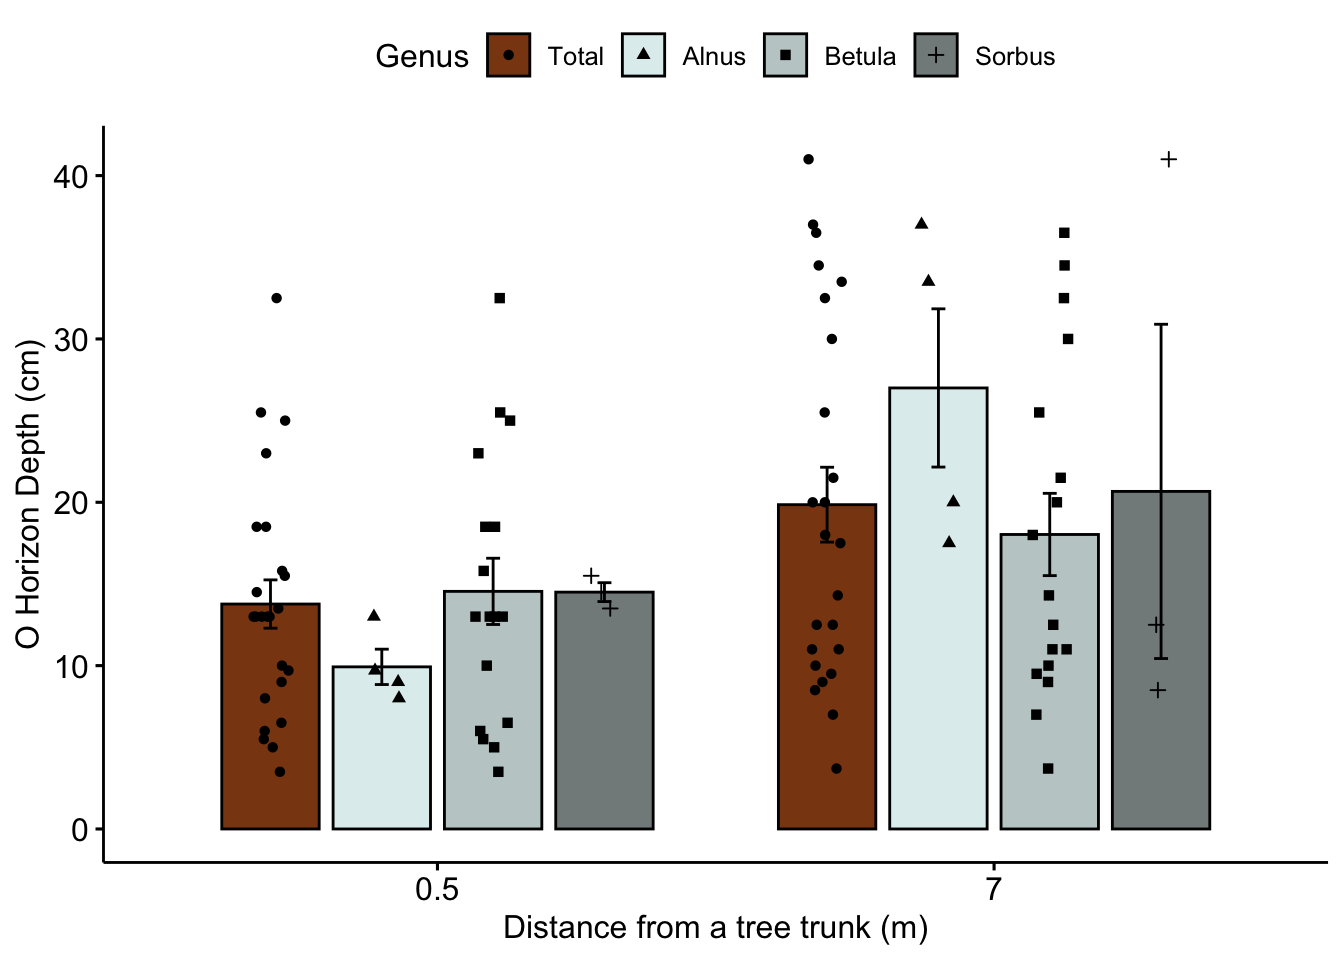
\includegraphics[keepaspectratio]{Soil_microclimate_EMproject_files/figure-latex/unnamed-chunk-6-1.pdf}}

\begin{Shaded}
\begin{Highlighting}[]
\FunctionTok{dev.off}\NormalTok{()}
\end{Highlighting}
\end{Shaded}

\begin{verbatim}
## null device 
##           1
\end{verbatim}

\section{Linear model: ANOVA for All tree \& Genus
specific}\label{linear-model-anova-for-all-tree-genus-specific}

\begin{Shaded}
\begin{Highlighting}[]
\CommentTok{\# All trees}
\DocumentationTok{\#\# ANOVA Depth vs. Distance{-}{-}{-}{-}}
\NormalTok{depth\_lm }\OtherTok{=} \FunctionTok{lm}\NormalTok{(Depth\_cm }\SpecialCharTok{\textasciitilde{}}\NormalTok{ Distance, }\AttributeTok{data =}\NormalTok{ soil\_all\_nonpine)}
\NormalTok{depth\_anov }\OtherTok{=} \FunctionTok{aov}\NormalTok{(depth\_lm, }\AttributeTok{data =}\NormalTok{ soil\_all\_nonpine)}

\NormalTok{table\_obj }\OtherTok{\textless{}{-}} \FunctionTok{tidy}\NormalTok{(depth\_anov)}
\FunctionTok{pander}\NormalTok{(depth\_anov, }\AttributeTok{digits =} \DecValTok{3}\NormalTok{)}
\end{Highlighting}
\end{Shaded}

\begin{longtable}[]{@{}
  >{\centering\arraybackslash}p{(\linewidth - 10\tabcolsep) * \real{0.2222}}
  >{\centering\arraybackslash}p{(\linewidth - 10\tabcolsep) * \real{0.0694}}
  >{\centering\arraybackslash}p{(\linewidth - 10\tabcolsep) * \real{0.1250}}
  >{\centering\arraybackslash}p{(\linewidth - 10\tabcolsep) * \real{0.1389}}
  >{\centering\arraybackslash}p{(\linewidth - 10\tabcolsep) * \real{0.1389}}
  >{\centering\arraybackslash}p{(\linewidth - 10\tabcolsep) * \real{0.1389}}@{}}
\caption{Analysis of Variance Model}\tabularnewline
\toprule\noalign{}
\begin{minipage}[b]{\linewidth}\centering
~
\end{minipage} & \begin{minipage}[b]{\linewidth}\centering
Df
\end{minipage} & \begin{minipage}[b]{\linewidth}\centering
Sum Sq
\end{minipage} & \begin{minipage}[b]{\linewidth}\centering
Mean Sq
\end{minipage} & \begin{minipage}[b]{\linewidth}\centering
F value
\end{minipage} & \begin{minipage}[b]{\linewidth}\centering
Pr(\textgreater F)
\end{minipage} \\
\midrule\noalign{}
\endfirsthead
\toprule\noalign{}
\begin{minipage}[b]{\linewidth}\centering
~
\end{minipage} & \begin{minipage}[b]{\linewidth}\centering
Df
\end{minipage} & \begin{minipage}[b]{\linewidth}\centering
Sum Sq
\end{minipage} & \begin{minipage}[b]{\linewidth}\centering
Mean Sq
\end{minipage} & \begin{minipage}[b]{\linewidth}\centering
F value
\end{minipage} & \begin{minipage}[b]{\linewidth}\centering
Pr(\textgreater F)
\end{minipage} \\
\midrule\noalign{}
\endhead
\bottomrule\noalign{}
\endlastfoot
\textbf{Distance} & 1 & 444 & 444 & 4.98 & 0.0306 \\
\textbf{Residuals} & 46 & 4104 & 89.2 & NA & NA \\
\end{longtable}

\begin{Shaded}
\begin{Highlighting}[]
\DocumentationTok{\#\# calculating mean}
\FunctionTok{tapply}\NormalTok{(soil\_all\_nonpine}\SpecialCharTok{$}\NormalTok{Depth\_cm, soil\_all\_nonpine}\SpecialCharTok{$}\NormalTok{Distance, mean, }\AttributeTok{na.rm=}\ConstantTok{TRUE}\NormalTok{)}
\end{Highlighting}
\end{Shaded}

\begin{verbatim}
##      0.5        7 
## 13.77083 19.85417
\end{verbatim}

\begin{Shaded}
\begin{Highlighting}[]
\DocumentationTok{\#\# Anscombe\textquotesingle{}s Quartet }
\FunctionTok{plot}\NormalTok{(depth\_lm) }
\end{Highlighting}
\end{Shaded}

\pandocbounded{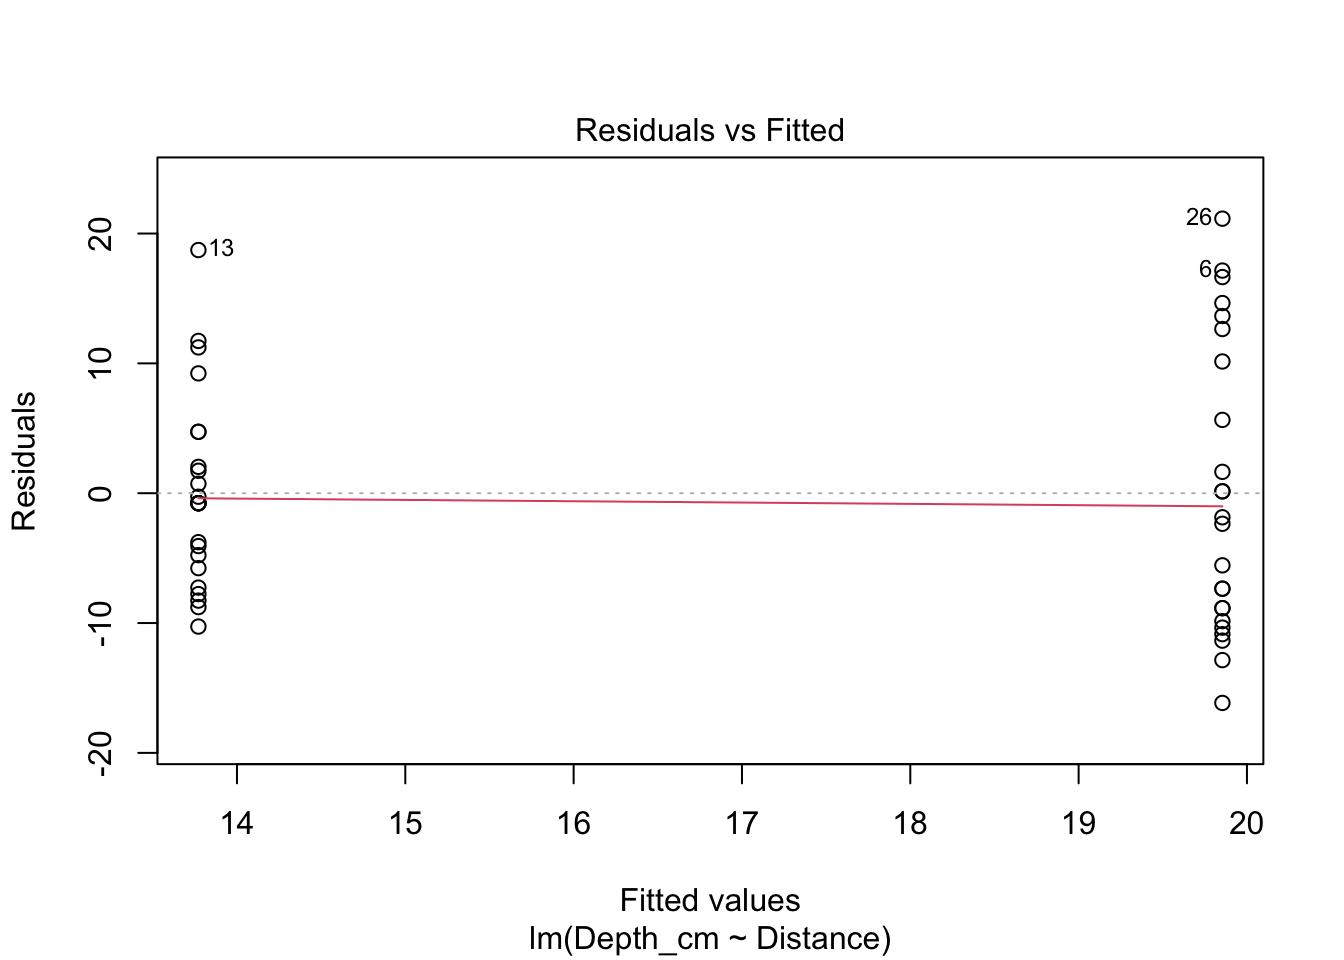
\includegraphics[keepaspectratio]{Soil_microclimate_EMproject_files/figure-latex/unnamed-chunk-7-1.pdf}}
\pandocbounded{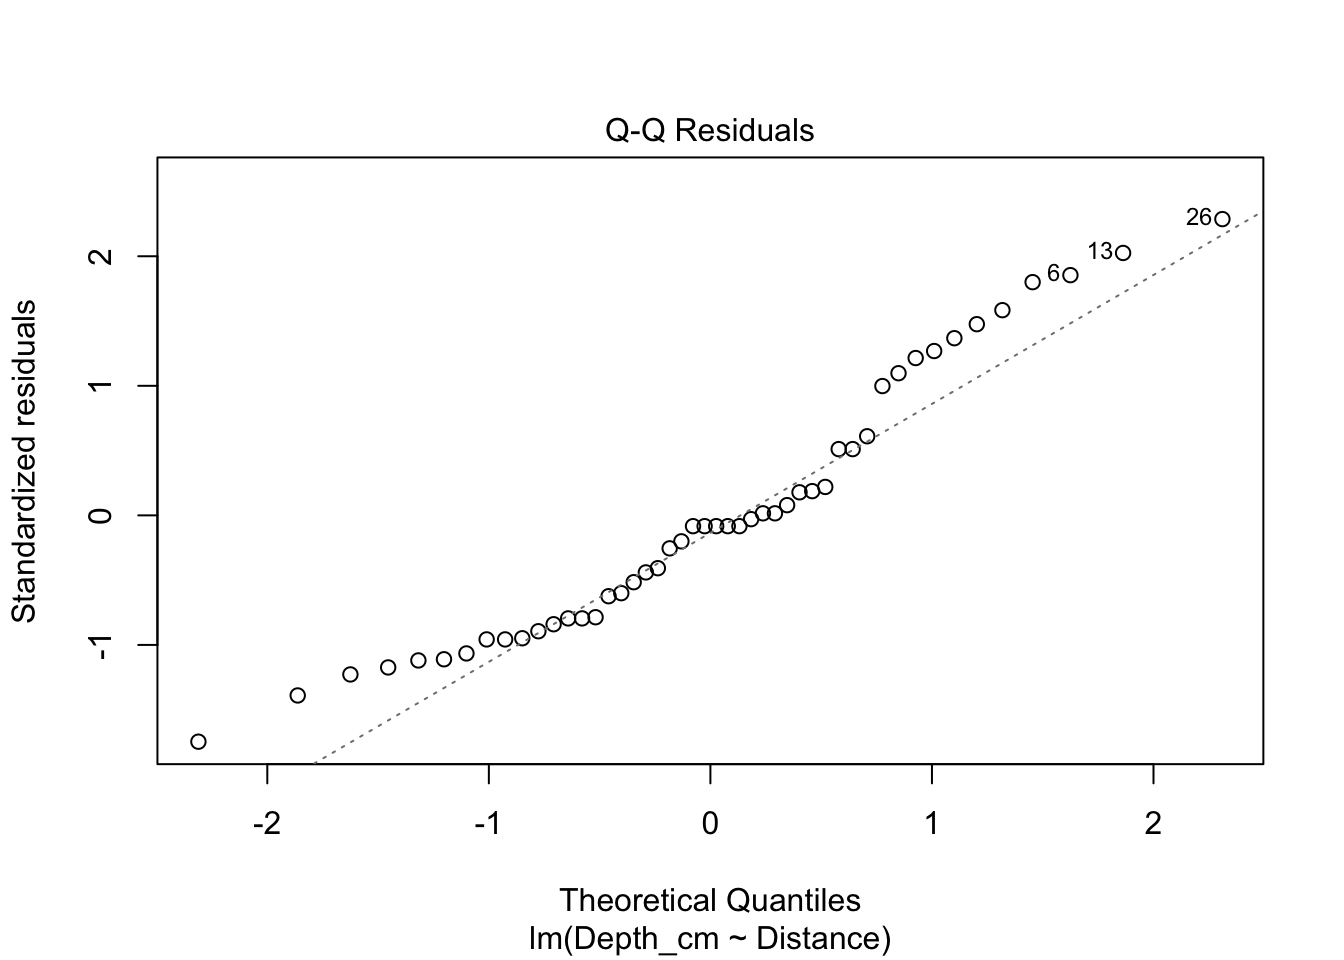
\includegraphics[keepaspectratio]{Soil_microclimate_EMproject_files/figure-latex/unnamed-chunk-7-2.pdf}}
\pandocbounded{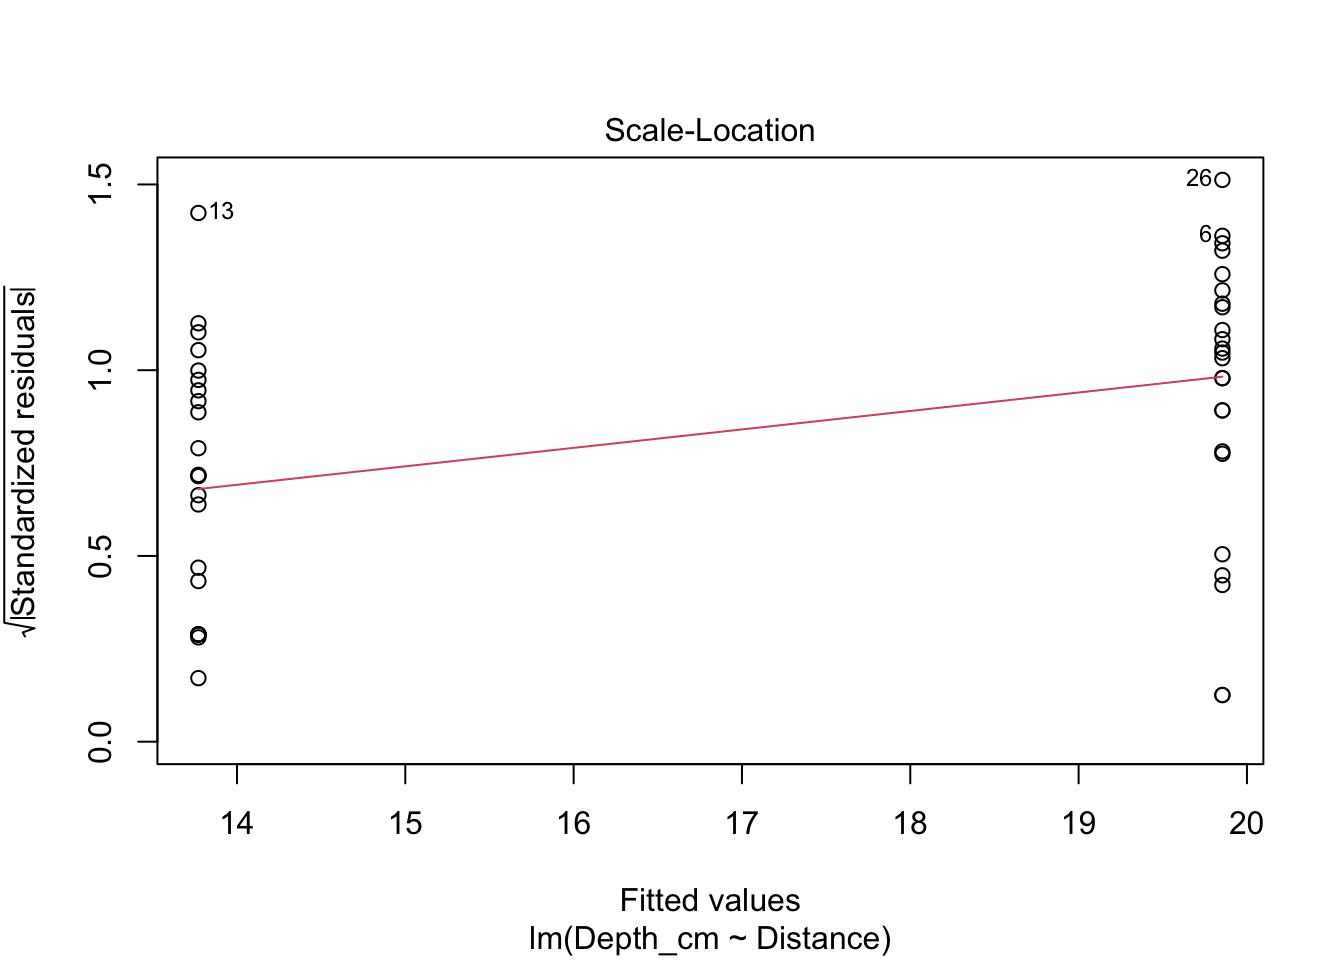
\includegraphics[keepaspectratio]{Soil_microclimate_EMproject_files/figure-latex/unnamed-chunk-7-3.pdf}}
\pandocbounded{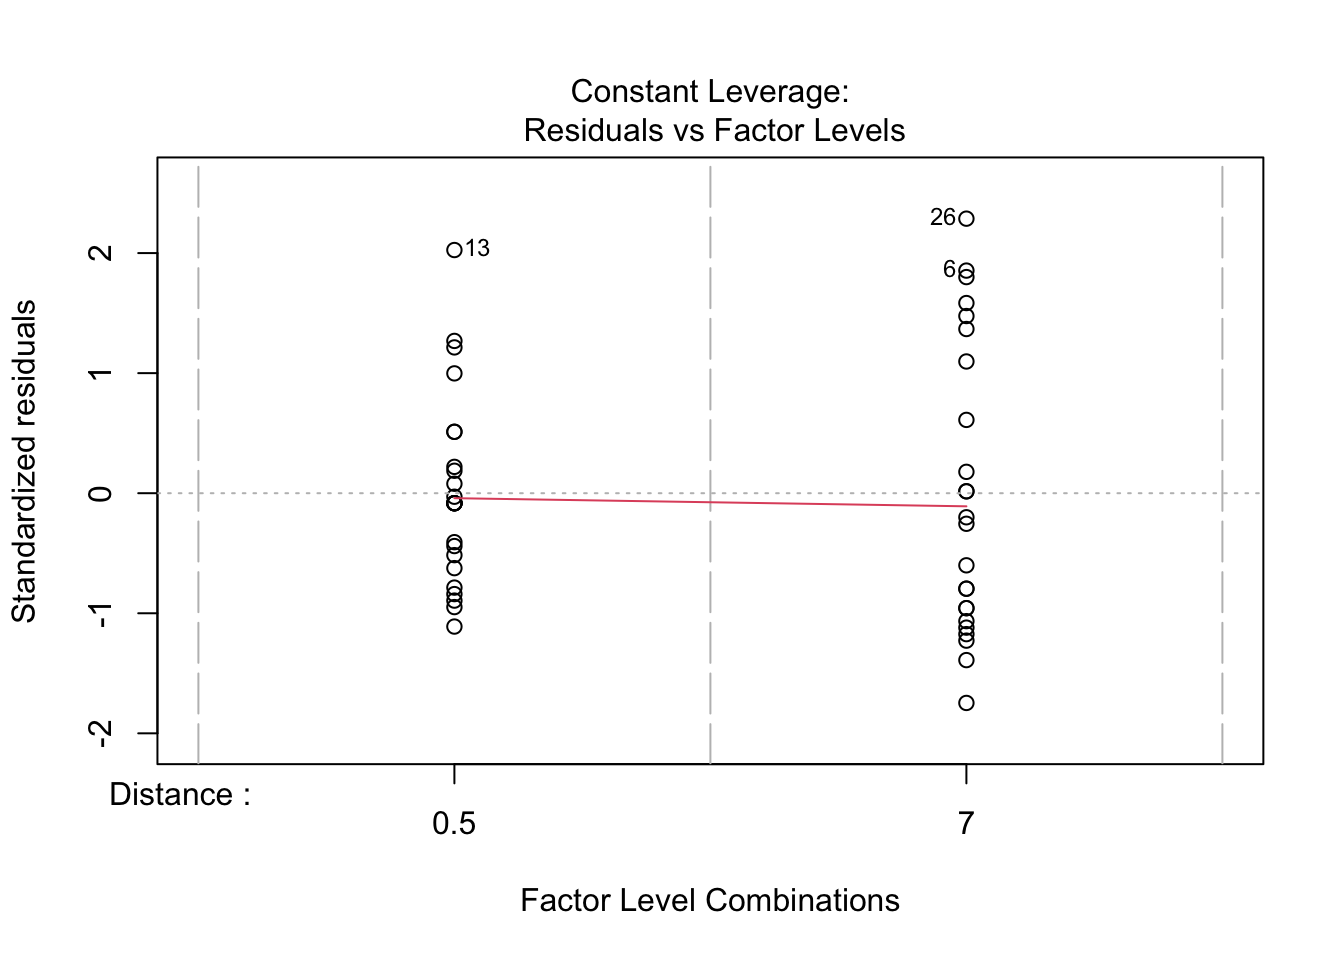
\includegraphics[keepaspectratio]{Soil_microclimate_EMproject_files/figure-latex/unnamed-chunk-7-4.pdf}}

\begin{Shaded}
\begin{Highlighting}[]
\CommentTok{\# Residuals vs. fitted: linearity met. }
\CommentTok{\# Q{-}Q plot generally follows the same line, residuals normally distributed. }
\CommentTok{\# Residuals variances are equal. }
\CommentTok{\# No significant outliers outside the Cook\textquotesingle{}s distance. }

\DocumentationTok{\#\# ANOVA Moisture vs. Distance{-}{-}{-}{-}}
\NormalTok{moisture\_lm }\OtherTok{\textless{}{-}} \FunctionTok{lm}\NormalTok{(Moisture\_vv }\SpecialCharTok{\textasciitilde{}}\NormalTok{ Distance, }\AttributeTok{data =}\NormalTok{ soil\_all\_nonpine)}
\NormalTok{moisture\_anov }\OtherTok{\textless{}{-}} \FunctionTok{aov}\NormalTok{(moisture\_lm)}

\NormalTok{table\_obj }\OtherTok{\textless{}{-}} \FunctionTok{tidy}\NormalTok{(moisture\_anov)}
\FunctionTok{pander}\NormalTok{(moisture\_anov, }\AttributeTok{digits =} \DecValTok{3}\NormalTok{)}
\end{Highlighting}
\end{Shaded}

\begin{longtable}[]{@{}
  >{\centering\arraybackslash}p{(\linewidth - 10\tabcolsep) * \real{0.2222}}
  >{\centering\arraybackslash}p{(\linewidth - 10\tabcolsep) * \real{0.0694}}
  >{\centering\arraybackslash}p{(\linewidth - 10\tabcolsep) * \real{0.1250}}
  >{\centering\arraybackslash}p{(\linewidth - 10\tabcolsep) * \real{0.1389}}
  >{\centering\arraybackslash}p{(\linewidth - 10\tabcolsep) * \real{0.1389}}
  >{\centering\arraybackslash}p{(\linewidth - 10\tabcolsep) * \real{0.1389}}@{}}
\caption{Analysis of Variance Model}\tabularnewline
\toprule\noalign{}
\begin{minipage}[b]{\linewidth}\centering
~
\end{minipage} & \begin{minipage}[b]{\linewidth}\centering
Df
\end{minipage} & \begin{minipage}[b]{\linewidth}\centering
Sum Sq
\end{minipage} & \begin{minipage}[b]{\linewidth}\centering
Mean Sq
\end{minipage} & \begin{minipage}[b]{\linewidth}\centering
F value
\end{minipage} & \begin{minipage}[b]{\linewidth}\centering
Pr(\textgreater F)
\end{minipage} \\
\midrule\noalign{}
\endfirsthead
\toprule\noalign{}
\begin{minipage}[b]{\linewidth}\centering
~
\end{minipage} & \begin{minipage}[b]{\linewidth}\centering
Df
\end{minipage} & \begin{minipage}[b]{\linewidth}\centering
Sum Sq
\end{minipage} & \begin{minipage}[b]{\linewidth}\centering
Mean Sq
\end{minipage} & \begin{minipage}[b]{\linewidth}\centering
F value
\end{minipage} & \begin{minipage}[b]{\linewidth}\centering
Pr(\textgreater F)
\end{minipage} \\
\midrule\noalign{}
\endhead
\bottomrule\noalign{}
\endlastfoot
\textbf{Distance} & 1 & 3323 & 3323 & 6.35 & 0.0153 \\
\textbf{Residuals} & 46 & 24086 & 524 & NA & NA \\
\end{longtable}

\begin{Shaded}
\begin{Highlighting}[]
\DocumentationTok{\#\# Anscombe\textquotesingle{}s Quartet }
\FunctionTok{plot}\NormalTok{(moisture\_lm)}
\end{Highlighting}
\end{Shaded}

\pandocbounded{\includegraphics[keepaspectratio]{Soil_microclimate_EMproject_files/figure-latex/unnamed-chunk-7-5.pdf}}
\pandocbounded{\includegraphics[keepaspectratio]{Soil_microclimate_EMproject_files/figure-latex/unnamed-chunk-7-6.pdf}}
\pandocbounded{\includegraphics[keepaspectratio]{Soil_microclimate_EMproject_files/figure-latex/unnamed-chunk-7-7.pdf}}
\pandocbounded{\includegraphics[keepaspectratio]{Soil_microclimate_EMproject_files/figure-latex/unnamed-chunk-7-8.pdf}}

\begin{Shaded}
\begin{Highlighting}[]
\CommentTok{\# Linearity met.}
\CommentTok{\# Q{-}Q plot generally follows the same line. }
\CommentTok{\# Residual variances are generally equal.}
\CommentTok{\# No significant outliers outside the Cook\textquotesingle{}s distance.}

\CommentTok{\# Species Specific }
\DocumentationTok{\#\# ANOVA Depth vs. Distance{-}{-}{-}{-}}
\DocumentationTok{\#\# Subset data for One{-}way ANOVA }
\NormalTok{Alnus }\OtherTok{\textless{}{-}} \FunctionTok{subset}\NormalTok{(soil\_all\_nonpine,Genus }\SpecialCharTok{==} \StringTok{"Alnus"}\NormalTok{)}
\NormalTok{Betula }\OtherTok{\textless{}{-}} \FunctionTok{subset}\NormalTok{(soil\_all\_nonpine, Genus }\SpecialCharTok{==} \StringTok{"Betula"}\NormalTok{)}
\NormalTok{Sorbus }\OtherTok{\textless{}{-}} \FunctionTok{subset}\NormalTok{(soil\_all\_nonpine, Genus }\SpecialCharTok{==} \StringTok{"Sorbus"}\NormalTok{)}

\DocumentationTok{\#\# ANOVA}
\NormalTok{alnus\_mod }\OtherTok{\textless{}{-}} \FunctionTok{aov}\NormalTok{(Depth\_cm }\SpecialCharTok{\textasciitilde{}}\NormalTok{ Distance, }\AttributeTok{data =}\NormalTok{ Alnus)}
\NormalTok{table\_obj }\OtherTok{\textless{}{-}} \FunctionTok{tidy}\NormalTok{(alnus\_mod)}
\FunctionTok{pander}\NormalTok{(alnus\_mod, }\AttributeTok{digits =} \DecValTok{3}\NormalTok{)}
\end{Highlighting}
\end{Shaded}

\begin{longtable}[]{@{}
  >{\centering\arraybackslash}p{(\linewidth - 10\tabcolsep) * \real{0.2222}}
  >{\centering\arraybackslash}p{(\linewidth - 10\tabcolsep) * \real{0.0694}}
  >{\centering\arraybackslash}p{(\linewidth - 10\tabcolsep) * \real{0.1250}}
  >{\centering\arraybackslash}p{(\linewidth - 10\tabcolsep) * \real{0.1389}}
  >{\centering\arraybackslash}p{(\linewidth - 10\tabcolsep) * \real{0.1389}}
  >{\centering\arraybackslash}p{(\linewidth - 10\tabcolsep) * \real{0.1389}}@{}}
\caption{Analysis of Variance Model}\tabularnewline
\toprule\noalign{}
\begin{minipage}[b]{\linewidth}\centering
~
\end{minipage} & \begin{minipage}[b]{\linewidth}\centering
Df
\end{minipage} & \begin{minipage}[b]{\linewidth}\centering
Sum Sq
\end{minipage} & \begin{minipage}[b]{\linewidth}\centering
Mean Sq
\end{minipage} & \begin{minipage}[b]{\linewidth}\centering
F value
\end{minipage} & \begin{minipage}[b]{\linewidth}\centering
Pr(\textgreater F)
\end{minipage} \\
\midrule\noalign{}
\endfirsthead
\toprule\noalign{}
\begin{minipage}[b]{\linewidth}\centering
~
\end{minipage} & \begin{minipage}[b]{\linewidth}\centering
Df
\end{minipage} & \begin{minipage}[b]{\linewidth}\centering
Sum Sq
\end{minipage} & \begin{minipage}[b]{\linewidth}\centering
Mean Sq
\end{minipage} & \begin{minipage}[b]{\linewidth}\centering
F value
\end{minipage} & \begin{minipage}[b]{\linewidth}\centering
Pr(\textgreater F)
\end{minipage} \\
\midrule\noalign{}
\endhead
\bottomrule\noalign{}
\endlastfoot
\textbf{Distance} & 1 & 583 & 583 & 11.8 & 0.0138 \\
\textbf{Residuals} & 6 & 296 & 49.3 & NA & NA \\
\end{longtable}

\begin{Shaded}
\begin{Highlighting}[]
\CommentTok{\# p = 0.01, df = 6. Significant difference. }
\NormalTok{betula\_mod }\OtherTok{\textless{}{-}} \FunctionTok{aov}\NormalTok{(Depth\_cm }\SpecialCharTok{\textasciitilde{}}\NormalTok{ Distance, }\AttributeTok{data =}\NormalTok{ Betula)}
\NormalTok{table\_obj }\OtherTok{\textless{}{-}} \FunctionTok{tidy}\NormalTok{(betula\_mod)}
\FunctionTok{pander}\NormalTok{(betula\_mod, }\AttributeTok{digits =} \DecValTok{3}\NormalTok{)}
\end{Highlighting}
\end{Shaded}

\begin{longtable}[]{@{}
  >{\centering\arraybackslash}p{(\linewidth - 10\tabcolsep) * \real{0.2222}}
  >{\centering\arraybackslash}p{(\linewidth - 10\tabcolsep) * \real{0.0694}}
  >{\centering\arraybackslash}p{(\linewidth - 10\tabcolsep) * \real{0.1250}}
  >{\centering\arraybackslash}p{(\linewidth - 10\tabcolsep) * \real{0.1389}}
  >{\centering\arraybackslash}p{(\linewidth - 10\tabcolsep) * \real{0.1389}}
  >{\centering\arraybackslash}p{(\linewidth - 10\tabcolsep) * \real{0.1389}}@{}}
\caption{Analysis of Variance Model}\tabularnewline
\toprule\noalign{}
\begin{minipage}[b]{\linewidth}\centering
~
\end{minipage} & \begin{minipage}[b]{\linewidth}\centering
Df
\end{minipage} & \begin{minipage}[b]{\linewidth}\centering
Sum Sq
\end{minipage} & \begin{minipage}[b]{\linewidth}\centering
Mean Sq
\end{minipage} & \begin{minipage}[b]{\linewidth}\centering
F value
\end{minipage} & \begin{minipage}[b]{\linewidth}\centering
Pr(\textgreater F)
\end{minipage} \\
\midrule\noalign{}
\endfirsthead
\toprule\noalign{}
\begin{minipage}[b]{\linewidth}\centering
~
\end{minipage} & \begin{minipage}[b]{\linewidth}\centering
Df
\end{minipage} & \begin{minipage}[b]{\linewidth}\centering
Sum Sq
\end{minipage} & \begin{minipage}[b]{\linewidth}\centering
Mean Sq
\end{minipage} & \begin{minipage}[b]{\linewidth}\centering
F value
\end{minipage} & \begin{minipage}[b]{\linewidth}\centering
Pr(\textgreater F)
\end{minipage} \\
\midrule\noalign{}
\endhead
\bottomrule\noalign{}
\endlastfoot
\textbf{Distance} & 1 & 103 & 103 & 1.16 & 0.29 \\
\textbf{Residuals} & 32 & 2845 & 88.9 & NA & NA \\
\end{longtable}

\begin{Shaded}
\begin{Highlighting}[]
\CommentTok{\# p = 0.29, df = 32, not significant. }
\NormalTok{sorbus\_mod }\OtherTok{\textless{}{-}} \FunctionTok{aov}\NormalTok{(Depth\_cm }\SpecialCharTok{\textasciitilde{}}\NormalTok{ Distance, }\AttributeTok{data =}\NormalTok{ Sorbus)}
\NormalTok{table\_obj }\OtherTok{\textless{}{-}} \FunctionTok{tidy}\NormalTok{(sorbus\_mod)}
\FunctionTok{pander}\NormalTok{(sorbus\_mod, }\AttributeTok{digits =} \DecValTok{3}\NormalTok{)}
\end{Highlighting}
\end{Shaded}

\begin{longtable}[]{@{}
  >{\centering\arraybackslash}p{(\linewidth - 10\tabcolsep) * \real{0.2222}}
  >{\centering\arraybackslash}p{(\linewidth - 10\tabcolsep) * \real{0.0694}}
  >{\centering\arraybackslash}p{(\linewidth - 10\tabcolsep) * \real{0.1250}}
  >{\centering\arraybackslash}p{(\linewidth - 10\tabcolsep) * \real{0.1389}}
  >{\centering\arraybackslash}p{(\linewidth - 10\tabcolsep) * \real{0.1389}}
  >{\centering\arraybackslash}p{(\linewidth - 10\tabcolsep) * \real{0.1389}}@{}}
\caption{Analysis of Variance Model}\tabularnewline
\toprule\noalign{}
\begin{minipage}[b]{\linewidth}\centering
~
\end{minipage} & \begin{minipage}[b]{\linewidth}\centering
Df
\end{minipage} & \begin{minipage}[b]{\linewidth}\centering
Sum Sq
\end{minipage} & \begin{minipage}[b]{\linewidth}\centering
Mean Sq
\end{minipage} & \begin{minipage}[b]{\linewidth}\centering
F value
\end{minipage} & \begin{minipage}[b]{\linewidth}\centering
Pr(\textgreater F)
\end{minipage} \\
\midrule\noalign{}
\endfirsthead
\toprule\noalign{}
\begin{minipage}[b]{\linewidth}\centering
~
\end{minipage} & \begin{minipage}[b]{\linewidth}\centering
Df
\end{minipage} & \begin{minipage}[b]{\linewidth}\centering
Sum Sq
\end{minipage} & \begin{minipage}[b]{\linewidth}\centering
Mean Sq
\end{minipage} & \begin{minipage}[b]{\linewidth}\centering
F value
\end{minipage} & \begin{minipage}[b]{\linewidth}\centering
Pr(\textgreater F)
\end{minipage} \\
\midrule\noalign{}
\endhead
\bottomrule\noalign{}
\endlastfoot
\textbf{Distance} & 1 & 57 & 57 & 0.362 & 0.58 \\
\textbf{Residuals} & 4 & 630 & 158 & NA & NA \\
\end{longtable}

\begin{Shaded}
\begin{Highlighting}[]
\CommentTok{\# p = 0.58, df = 4, not significant. }

\DocumentationTok{\#\# ANOVA Moisture vs. Distance{-}{-}{-}{-}}

\DocumentationTok{\#\# ANOVA}
\NormalTok{alnus\_mod }\OtherTok{\textless{}{-}} \FunctionTok{aov}\NormalTok{(Moisture\_vv }\SpecialCharTok{\textasciitilde{}}\NormalTok{ Distance, }\AttributeTok{data =}\NormalTok{ Alnus)}
\NormalTok{table\_obj }\OtherTok{\textless{}{-}} \FunctionTok{tidy}\NormalTok{(alnus\_mod)}
\FunctionTok{pander}\NormalTok{(alnus\_mod, }\AttributeTok{digits =} \DecValTok{3}\NormalTok{)}
\end{Highlighting}
\end{Shaded}

\begin{longtable}[]{@{}
  >{\centering\arraybackslash}p{(\linewidth - 10\tabcolsep) * \real{0.2222}}
  >{\centering\arraybackslash}p{(\linewidth - 10\tabcolsep) * \real{0.0694}}
  >{\centering\arraybackslash}p{(\linewidth - 10\tabcolsep) * \real{0.1250}}
  >{\centering\arraybackslash}p{(\linewidth - 10\tabcolsep) * \real{0.1389}}
  >{\centering\arraybackslash}p{(\linewidth - 10\tabcolsep) * \real{0.1389}}
  >{\centering\arraybackslash}p{(\linewidth - 10\tabcolsep) * \real{0.1389}}@{}}
\caption{Analysis of Variance Model}\tabularnewline
\toprule\noalign{}
\begin{minipage}[b]{\linewidth}\centering
~
\end{minipage} & \begin{minipage}[b]{\linewidth}\centering
Df
\end{minipage} & \begin{minipage}[b]{\linewidth}\centering
Sum Sq
\end{minipage} & \begin{minipage}[b]{\linewidth}\centering
Mean Sq
\end{minipage} & \begin{minipage}[b]{\linewidth}\centering
F value
\end{minipage} & \begin{minipage}[b]{\linewidth}\centering
Pr(\textgreater F)
\end{minipage} \\
\midrule\noalign{}
\endfirsthead
\toprule\noalign{}
\begin{minipage}[b]{\linewidth}\centering
~
\end{minipage} & \begin{minipage}[b]{\linewidth}\centering
Df
\end{minipage} & \begin{minipage}[b]{\linewidth}\centering
Sum Sq
\end{minipage} & \begin{minipage}[b]{\linewidth}\centering
Mean Sq
\end{minipage} & \begin{minipage}[b]{\linewidth}\centering
F value
\end{minipage} & \begin{minipage}[b]{\linewidth}\centering
Pr(\textgreater F)
\end{minipage} \\
\midrule\noalign{}
\endhead
\bottomrule\noalign{}
\endlastfoot
\textbf{Distance} & 1 & 2468 & 2468 & 4.48 & 0.0788 \\
\textbf{Residuals} & 6 & 3308 & 551 & NA & NA \\
\end{longtable}

\begin{Shaded}
\begin{Highlighting}[]
\CommentTok{\# p = 0.08, df = 6. not significant. }
\NormalTok{betula\_mod }\OtherTok{\textless{}{-}} \FunctionTok{aov}\NormalTok{(Moisture\_vv }\SpecialCharTok{\textasciitilde{}}\NormalTok{ Distance, }\AttributeTok{data =}\NormalTok{ Betula)}
\NormalTok{table\_obj }\OtherTok{\textless{}{-}} \FunctionTok{tidy}\NormalTok{(betula\_mod)}
\FunctionTok{pander}\NormalTok{(betula\_mod, }\AttributeTok{digits =} \DecValTok{3}\NormalTok{)}
\end{Highlighting}
\end{Shaded}

\begin{longtable}[]{@{}
  >{\centering\arraybackslash}p{(\linewidth - 10\tabcolsep) * \real{0.2222}}
  >{\centering\arraybackslash}p{(\linewidth - 10\tabcolsep) * \real{0.0694}}
  >{\centering\arraybackslash}p{(\linewidth - 10\tabcolsep) * \real{0.1250}}
  >{\centering\arraybackslash}p{(\linewidth - 10\tabcolsep) * \real{0.1389}}
  >{\centering\arraybackslash}p{(\linewidth - 10\tabcolsep) * \real{0.1389}}
  >{\centering\arraybackslash}p{(\linewidth - 10\tabcolsep) * \real{0.1389}}@{}}
\caption{Analysis of Variance Model}\tabularnewline
\toprule\noalign{}
\begin{minipage}[b]{\linewidth}\centering
~
\end{minipage} & \begin{minipage}[b]{\linewidth}\centering
Df
\end{minipage} & \begin{minipage}[b]{\linewidth}\centering
Sum Sq
\end{minipage} & \begin{minipage}[b]{\linewidth}\centering
Mean Sq
\end{minipage} & \begin{minipage}[b]{\linewidth}\centering
F value
\end{minipage} & \begin{minipage}[b]{\linewidth}\centering
Pr(\textgreater F)
\end{minipage} \\
\midrule\noalign{}
\endfirsthead
\toprule\noalign{}
\begin{minipage}[b]{\linewidth}\centering
~
\end{minipage} & \begin{minipage}[b]{\linewidth}\centering
Df
\end{minipage} & \begin{minipage}[b]{\linewidth}\centering
Sum Sq
\end{minipage} & \begin{minipage}[b]{\linewidth}\centering
Mean Sq
\end{minipage} & \begin{minipage}[b]{\linewidth}\centering
F value
\end{minipage} & \begin{minipage}[b]{\linewidth}\centering
Pr(\textgreater F)
\end{minipage} \\
\midrule\noalign{}
\endhead
\bottomrule\noalign{}
\endlastfoot
\textbf{Distance} & 1 & 1171 & 1171 & 2.25 & 0.144 \\
\textbf{Residuals} & 32 & 16681 & 521 & NA & NA \\
\end{longtable}

\begin{Shaded}
\begin{Highlighting}[]
\CommentTok{\# p = 0.14, df = 32, not significant. }
\NormalTok{sorbus\_mod }\OtherTok{\textless{}{-}} \FunctionTok{aov}\NormalTok{(Moisture\_vv }\SpecialCharTok{\textasciitilde{}}\NormalTok{ Distance, }\AttributeTok{data =}\NormalTok{ Sorbus)}
\NormalTok{table\_obj }\OtherTok{\textless{}{-}} \FunctionTok{tidy}\NormalTok{(sorbus\_mod)}
\FunctionTok{pander}\NormalTok{(sorbus\_mod, }\AttributeTok{digits =} \DecValTok{3}\NormalTok{)}
\end{Highlighting}
\end{Shaded}

\begin{longtable}[]{@{}
  >{\centering\arraybackslash}p{(\linewidth - 10\tabcolsep) * \real{0.2222}}
  >{\centering\arraybackslash}p{(\linewidth - 10\tabcolsep) * \real{0.0694}}
  >{\centering\arraybackslash}p{(\linewidth - 10\tabcolsep) * \real{0.1250}}
  >{\centering\arraybackslash}p{(\linewidth - 10\tabcolsep) * \real{0.1389}}
  >{\centering\arraybackslash}p{(\linewidth - 10\tabcolsep) * \real{0.1389}}
  >{\centering\arraybackslash}p{(\linewidth - 10\tabcolsep) * \real{0.1389}}@{}}
\caption{Analysis of Variance Model}\tabularnewline
\toprule\noalign{}
\begin{minipage}[b]{\linewidth}\centering
~
\end{minipage} & \begin{minipage}[b]{\linewidth}\centering
Df
\end{minipage} & \begin{minipage}[b]{\linewidth}\centering
Sum Sq
\end{minipage} & \begin{minipage}[b]{\linewidth}\centering
Mean Sq
\end{minipage} & \begin{minipage}[b]{\linewidth}\centering
F value
\end{minipage} & \begin{minipage}[b]{\linewidth}\centering
Pr(\textgreater F)
\end{minipage} \\
\midrule\noalign{}
\endfirsthead
\toprule\noalign{}
\begin{minipage}[b]{\linewidth}\centering
~
\end{minipage} & \begin{minipage}[b]{\linewidth}\centering
Df
\end{minipage} & \begin{minipage}[b]{\linewidth}\centering
Sum Sq
\end{minipage} & \begin{minipage}[b]{\linewidth}\centering
Mean Sq
\end{minipage} & \begin{minipage}[b]{\linewidth}\centering
F value
\end{minipage} & \begin{minipage}[b]{\linewidth}\centering
Pr(\textgreater F)
\end{minipage} \\
\midrule\noalign{}
\endhead
\bottomrule\noalign{}
\endlastfoot
\textbf{Distance} & 1 & 588 & 588 & 0.985 & 0.377 \\
\textbf{Residuals} & 4 & 2389 & 597 & NA & NA \\
\end{longtable}

\begin{Shaded}
\begin{Highlighting}[]
\CommentTok{\# p = 0.38, df = 4, not significant. }
\end{Highlighting}
\end{Shaded}

\section{Visualisation: Management
specific}\label{visualisation-management-specific}

\begin{Shaded}
\begin{Highlighting}[]
\DocumentationTok{\#\# Distance vs O Horizon depth (cm)}
\NormalTok{p3 }\OtherTok{\textless{}{-}} \FunctionTok{ggbarplot}\NormalTok{(}
\NormalTok{  soil\_all\_nonpine, }\AttributeTok{x =} \StringTok{"Distance"}\NormalTok{, }\AttributeTok{y =} \StringTok{"Depth\_cm"}\NormalTok{, }
  \AttributeTok{add =} \FunctionTok{c}\NormalTok{(}\StringTok{"mean\_se"}\NormalTok{, }\StringTok{"jitter"}\NormalTok{), }
  \AttributeTok{add.params =} \FunctionTok{list}\NormalTok{(}\AttributeTok{shape =} \StringTok{"Management"}\NormalTok{),}
  \AttributeTok{fill=} \StringTok{"Management"}\NormalTok{, }\AttributeTok{palette =} \FunctionTok{c}\NormalTok{(}
    \StringTok{"No mound"} \OtherTok{=} \StringTok{"\#D9C2C1"}\NormalTok{, }
    \StringTok{"mound"} \OtherTok{=} \StringTok{"gray"}\NormalTok{),}
  \AttributeTok{position =} \FunctionTok{position\_dodge}\NormalTok{(}\FloatTok{0.8}\NormalTok{)}
\NormalTok{) }\SpecialCharTok{+} 
  \FunctionTok{labs}\NormalTok{(}\AttributeTok{x =} \StringTok{"Distance from a tree trunk (m)"}\NormalTok{, }\AttributeTok{y =} \StringTok{"O Horizon Depth (cm)"}\NormalTok{)}

\DocumentationTok{\#\# Distance vs Soil moisture (cm)}
\NormalTok{p4 }\OtherTok{\textless{}{-}} \FunctionTok{ggbarplot}\NormalTok{(}
\NormalTok{  soil\_all\_nonpine, }\AttributeTok{x =} \StringTok{"Distance"}\NormalTok{, }\AttributeTok{y =} \StringTok{"Moisture\_vv"}\NormalTok{, }
  \AttributeTok{add =} \FunctionTok{c}\NormalTok{(}\StringTok{"mean\_se"}\NormalTok{, }\StringTok{"jitter"}\NormalTok{), }
  \AttributeTok{add.params =} \FunctionTok{list}\NormalTok{(}\AttributeTok{shape =} \StringTok{"Management"}\NormalTok{),}
  \AttributeTok{fill=} \StringTok{"Management"}\NormalTok{, }\AttributeTok{palette =} \FunctionTok{c}\NormalTok{(}
    \StringTok{"No mound"} \OtherTok{=} \StringTok{"\#A7B9E8"}\NormalTok{, }
    \StringTok{"mound"} \OtherTok{=} \StringTok{"gray"}\NormalTok{),}
  \AttributeTok{position =} \FunctionTok{position\_dodge}\NormalTok{(}\FloatTok{0.8}\NormalTok{)}
\NormalTok{) }\SpecialCharTok{+} 
  \FunctionTok{labs}\NormalTok{(}\AttributeTok{x =} \StringTok{"Distance from a tree trunk (m)"}\NormalTok{, }\AttributeTok{y =} \StringTok{"Soil moisture (\%, v/v)"}\NormalTok{)}

\FunctionTok{ggarrange}\NormalTok{(}
\NormalTok{  p3, p4,}
  \AttributeTok{labels =} \FunctionTok{c}\NormalTok{(}\StringTok{"a"}\NormalTok{, }\StringTok{"b"}\NormalTok{),}
  \AttributeTok{ncol =} \DecValTok{2}\NormalTok{, }\AttributeTok{nrow =} \DecValTok{1}\NormalTok{,}
  \AttributeTok{common.legend =} \ConstantTok{FALSE}
\NormalTok{)}
\end{Highlighting}
\end{Shaded}

\pandocbounded{\includegraphics[keepaspectratio]{Soil_microclimate_EMproject_files/figure-latex/unnamed-chunk-8-1.pdf}}

\section{Linear model: ANOVA for Management
specific}\label{linear-model-anova-for-management-specific}

\begin{Shaded}
\begin{Highlighting}[]
\CommentTok{\# Subset data}
\NormalTok{no\_mound }\OtherTok{\textless{}{-}}\NormalTok{ soil\_all\_nonpine }\SpecialCharTok{\%\textgreater{}\%}
  \FunctionTok{subset}\NormalTok{(Management }\SpecialCharTok{==} \StringTok{"No mound"}\NormalTok{)}
\NormalTok{mound }\OtherTok{\textless{}{-}}\NormalTok{ soil\_all\_nonpine }\SpecialCharTok{\%\textgreater{}\%}
  \FunctionTok{subset}\NormalTok{(Management }\SpecialCharTok{==} \StringTok{"mound"}\NormalTok{)}

\CommentTok{\# ANOVA}
\DocumentationTok{\#\# Depth vs. Distance {-}{-}{-}{-}}
\DocumentationTok{\#\#\# Mound}
\NormalTok{mound\_aov }\OtherTok{\textless{}{-}} \FunctionTok{aov}\NormalTok{(Depth\_cm }\SpecialCharTok{\textasciitilde{}}\NormalTok{ Distance, }\AttributeTok{data =}\NormalTok{ mound)}
\NormalTok{table\_obj }\OtherTok{\textless{}{-}} \FunctionTok{tidy}\NormalTok{(mound\_aov)}
\FunctionTok{pander}\NormalTok{(mound\_aov, }\AttributeTok{digits =} \DecValTok{3}\NormalTok{)}
\end{Highlighting}
\end{Shaded}

\begin{longtable}[]{@{}
  >{\centering\arraybackslash}p{(\linewidth - 10\tabcolsep) * \real{0.2222}}
  >{\centering\arraybackslash}p{(\linewidth - 10\tabcolsep) * \real{0.0694}}
  >{\centering\arraybackslash}p{(\linewidth - 10\tabcolsep) * \real{0.1250}}
  >{\centering\arraybackslash}p{(\linewidth - 10\tabcolsep) * \real{0.1389}}
  >{\centering\arraybackslash}p{(\linewidth - 10\tabcolsep) * \real{0.1389}}
  >{\centering\arraybackslash}p{(\linewidth - 10\tabcolsep) * \real{0.1389}}@{}}
\caption{Analysis of Variance Model}\tabularnewline
\toprule\noalign{}
\begin{minipage}[b]{\linewidth}\centering
~
\end{minipage} & \begin{minipage}[b]{\linewidth}\centering
Df
\end{minipage} & \begin{minipage}[b]{\linewidth}\centering
Sum Sq
\end{minipage} & \begin{minipage}[b]{\linewidth}\centering
Mean Sq
\end{minipage} & \begin{minipage}[b]{\linewidth}\centering
F value
\end{minipage} & \begin{minipage}[b]{\linewidth}\centering
Pr(\textgreater F)
\end{minipage} \\
\midrule\noalign{}
\endfirsthead
\toprule\noalign{}
\begin{minipage}[b]{\linewidth}\centering
~
\end{minipage} & \begin{minipage}[b]{\linewidth}\centering
Df
\end{minipage} & \begin{minipage}[b]{\linewidth}\centering
Sum Sq
\end{minipage} & \begin{minipage}[b]{\linewidth}\centering
Mean Sq
\end{minipage} & \begin{minipage}[b]{\linewidth}\centering
F value
\end{minipage} & \begin{minipage}[b]{\linewidth}\centering
Pr(\textgreater F)
\end{minipage} \\
\midrule\noalign{}
\endhead
\bottomrule\noalign{}
\endlastfoot
\textbf{Distance} & 1 & 372 & 372 & 5.46 & 0.0289 \\
\textbf{Residuals} & 22 & 1498 & 68.1 & NA & NA \\
\end{longtable}

\begin{Shaded}
\begin{Highlighting}[]
\DocumentationTok{\#\#\# No mound}
\NormalTok{no\_mound\_aov }\OtherTok{\textless{}{-}} \FunctionTok{aov}\NormalTok{(Depth\_cm }\SpecialCharTok{\textasciitilde{}}\NormalTok{ Distance, }\AttributeTok{data =}\NormalTok{ no\_mound)}
\NormalTok{table\_obj }\OtherTok{\textless{}{-}} \FunctionTok{tidy}\NormalTok{(no\_mound\_aov)}
\FunctionTok{pander}\NormalTok{(no\_mound\_aov, }\AttributeTok{digits =} \DecValTok{3}\NormalTok{)}
\end{Highlighting}
\end{Shaded}

\begin{longtable}[]{@{}
  >{\centering\arraybackslash}p{(\linewidth - 10\tabcolsep) * \real{0.2222}}
  >{\centering\arraybackslash}p{(\linewidth - 10\tabcolsep) * \real{0.0694}}
  >{\centering\arraybackslash}p{(\linewidth - 10\tabcolsep) * \real{0.1250}}
  >{\centering\arraybackslash}p{(\linewidth - 10\tabcolsep) * \real{0.1389}}
  >{\centering\arraybackslash}p{(\linewidth - 10\tabcolsep) * \real{0.1389}}
  >{\centering\arraybackslash}p{(\linewidth - 10\tabcolsep) * \real{0.1389}}@{}}
\caption{Analysis of Variance Model}\tabularnewline
\toprule\noalign{}
\begin{minipage}[b]{\linewidth}\centering
~
\end{minipage} & \begin{minipage}[b]{\linewidth}\centering
Df
\end{minipage} & \begin{minipage}[b]{\linewidth}\centering
Sum Sq
\end{minipage} & \begin{minipage}[b]{\linewidth}\centering
Mean Sq
\end{minipage} & \begin{minipage}[b]{\linewidth}\centering
F value
\end{minipage} & \begin{minipage}[b]{\linewidth}\centering
Pr(\textgreater F)
\end{minipage} \\
\midrule\noalign{}
\endfirsthead
\toprule\noalign{}
\begin{minipage}[b]{\linewidth}\centering
~
\end{minipage} & \begin{minipage}[b]{\linewidth}\centering
Df
\end{minipage} & \begin{minipage}[b]{\linewidth}\centering
Sum Sq
\end{minipage} & \begin{minipage}[b]{\linewidth}\centering
Mean Sq
\end{minipage} & \begin{minipage}[b]{\linewidth}\centering
F value
\end{minipage} & \begin{minipage}[b]{\linewidth}\centering
Pr(\textgreater F)
\end{minipage} \\
\midrule\noalign{}
\endhead
\bottomrule\noalign{}
\endlastfoot
\textbf{Distance} & 1 & 111 & 111 & 0.956 & 0.339 \\
\textbf{Residuals} & 22 & 2542 & 116 & NA & NA \\
\end{longtable}

\begin{Shaded}
\begin{Highlighting}[]
\CommentTok{\# p = 0.05 for mound, p = 0.34 for no{-}mound.}
\CommentTok{\# df = 24, and df = 24, respectively. }

\DocumentationTok{\#\# Moisture vs. Distance {-}{-}{-}{-}}
\DocumentationTok{\#\#\# Mound}
\NormalTok{mound\_aov }\OtherTok{\textless{}{-}} \FunctionTok{aov}\NormalTok{(Moisture\_vv }\SpecialCharTok{\textasciitilde{}}\NormalTok{ Distance, }\AttributeTok{data =}\NormalTok{ mound)}
\NormalTok{table\_obj }\OtherTok{\textless{}{-}} \FunctionTok{tidy}\NormalTok{(mound\_aov)}
\FunctionTok{pander}\NormalTok{(mound\_aov, }\AttributeTok{digits =} \DecValTok{3}\NormalTok{)}
\end{Highlighting}
\end{Shaded}

\begin{longtable}[]{@{}
  >{\centering\arraybackslash}p{(\linewidth - 10\tabcolsep) * \real{0.2222}}
  >{\centering\arraybackslash}p{(\linewidth - 10\tabcolsep) * \real{0.0694}}
  >{\centering\arraybackslash}p{(\linewidth - 10\tabcolsep) * \real{0.1250}}
  >{\centering\arraybackslash}p{(\linewidth - 10\tabcolsep) * \real{0.1389}}
  >{\centering\arraybackslash}p{(\linewidth - 10\tabcolsep) * \real{0.1389}}
  >{\centering\arraybackslash}p{(\linewidth - 10\tabcolsep) * \real{0.1389}}@{}}
\caption{Analysis of Variance Model}\tabularnewline
\toprule\noalign{}
\begin{minipage}[b]{\linewidth}\centering
~
\end{minipage} & \begin{minipage}[b]{\linewidth}\centering
Df
\end{minipage} & \begin{minipage}[b]{\linewidth}\centering
Sum Sq
\end{minipage} & \begin{minipage}[b]{\linewidth}\centering
Mean Sq
\end{minipage} & \begin{minipage}[b]{\linewidth}\centering
F value
\end{minipage} & \begin{minipage}[b]{\linewidth}\centering
Pr(\textgreater F)
\end{minipage} \\
\midrule\noalign{}
\endfirsthead
\toprule\noalign{}
\begin{minipage}[b]{\linewidth}\centering
~
\end{minipage} & \begin{minipage}[b]{\linewidth}\centering
Df
\end{minipage} & \begin{minipage}[b]{\linewidth}\centering
Sum Sq
\end{minipage} & \begin{minipage}[b]{\linewidth}\centering
Mean Sq
\end{minipage} & \begin{minipage}[b]{\linewidth}\centering
F value
\end{minipage} & \begin{minipage}[b]{\linewidth}\centering
Pr(\textgreater F)
\end{minipage} \\
\midrule\noalign{}
\endhead
\bottomrule\noalign{}
\endlastfoot
\textbf{Distance} & 1 & 1190 & 1190 & 1.88 & 0.184 \\
\textbf{Residuals} & 22 & 13898 & 632 & NA & NA \\
\end{longtable}

\begin{Shaded}
\begin{Highlighting}[]
\DocumentationTok{\#\#\# No mound }
\NormalTok{no\_mound\_aov }\OtherTok{\textless{}{-}} \FunctionTok{aov}\NormalTok{(Moisture\_vv }\SpecialCharTok{\textasciitilde{}}\NormalTok{ Distance, }\AttributeTok{data =}\NormalTok{ no\_mound)}
\NormalTok{table\_obj }\OtherTok{\textless{}{-}} \FunctionTok{tidy}\NormalTok{(no\_mound\_aov)}
\FunctionTok{pander}\NormalTok{(no\_mound\_aov, }\AttributeTok{digits =} \DecValTok{3}\NormalTok{)}
\end{Highlighting}
\end{Shaded}

\begin{longtable}[]{@{}
  >{\centering\arraybackslash}p{(\linewidth - 10\tabcolsep) * \real{0.2222}}
  >{\centering\arraybackslash}p{(\linewidth - 10\tabcolsep) * \real{0.0694}}
  >{\centering\arraybackslash}p{(\linewidth - 10\tabcolsep) * \real{0.1250}}
  >{\centering\arraybackslash}p{(\linewidth - 10\tabcolsep) * \real{0.1389}}
  >{\centering\arraybackslash}p{(\linewidth - 10\tabcolsep) * \real{0.1389}}
  >{\centering\arraybackslash}p{(\linewidth - 10\tabcolsep) * \real{0.1389}}@{}}
\caption{Analysis of Variance Model}\tabularnewline
\toprule\noalign{}
\begin{minipage}[b]{\linewidth}\centering
~
\end{minipage} & \begin{minipage}[b]{\linewidth}\centering
Df
\end{minipage} & \begin{minipage}[b]{\linewidth}\centering
Sum Sq
\end{minipage} & \begin{minipage}[b]{\linewidth}\centering
Mean Sq
\end{minipage} & \begin{minipage}[b]{\linewidth}\centering
F value
\end{minipage} & \begin{minipage}[b]{\linewidth}\centering
Pr(\textgreater F)
\end{minipage} \\
\midrule\noalign{}
\endfirsthead
\toprule\noalign{}
\begin{minipage}[b]{\linewidth}\centering
~
\end{minipage} & \begin{minipage}[b]{\linewidth}\centering
Df
\end{minipage} & \begin{minipage}[b]{\linewidth}\centering
Sum Sq
\end{minipage} & \begin{minipage}[b]{\linewidth}\centering
Mean Sq
\end{minipage} & \begin{minipage}[b]{\linewidth}\centering
F value
\end{minipage} & \begin{minipage}[b]{\linewidth}\centering
Pr(\textgreater F)
\end{minipage} \\
\midrule\noalign{}
\endhead
\bottomrule\noalign{}
\endlastfoot
\textbf{Distance} & 1 & 2212 & 2212 & 4.91 & 0.0373 \\
\textbf{Residuals} & 22 & 9905 & 450 & NA & NA \\
\end{longtable}

\begin{Shaded}
\begin{Highlighting}[]
\CommentTok{\# p = 0.22 for mound, p = 0.04 for no{-}mound. }
\CommentTok{\# df = 24 and df = 24 respectively.}
\end{Highlighting}
\end{Shaded}

\section{Means ± SEs for ALL Groups}\label{means-ses-for-all-groups}

\begin{Shaded}
\begin{Highlighting}[]
\CommentTok{\# total trees }
\NormalTok{total\_summary }\OtherTok{\textless{}{-}}\NormalTok{ soil\_all\_nonpine }\SpecialCharTok{\%\textgreater{}\%}
  \FunctionTok{group\_by}\NormalTok{(Distance) }\SpecialCharTok{\%\textgreater{}\%}
   \FunctionTok{summarise}\NormalTok{(}
    \AttributeTok{Mean\_depth =} \FunctionTok{mean}\NormalTok{(Depth\_cm, }\AttributeTok{na.rm =} \ConstantTok{TRUE}\NormalTok{),}
    \AttributeTok{SE\_depth   =} \FunctionTok{sd}\NormalTok{(Depth\_cm, }\AttributeTok{na.rm =} \ConstantTok{TRUE}\NormalTok{) }\SpecialCharTok{/} \FunctionTok{sqrt}\NormalTok{(}\FunctionTok{n}\NormalTok{()), }
    \AttributeTok{Mean\_moist =} \FunctionTok{mean}\NormalTok{(Moisture\_vv, }\AttributeTok{na.rm =} \ConstantTok{TRUE}\NormalTok{),}
    \AttributeTok{SE\_moist   =} \FunctionTok{sd}\NormalTok{(Moisture\_vv, }\AttributeTok{na.rm =} \ConstantTok{TRUE}\NormalTok{) }\SpecialCharTok{/} \FunctionTok{sqrt}\NormalTok{(}\FunctionTok{n}\NormalTok{())}
\NormalTok{  )}
\CommentTok{\# grouped by genus}
\NormalTok{genus\_summary }\OtherTok{\textless{}{-}}\NormalTok{ soil\_all\_nonpine }\SpecialCharTok{\%\textgreater{}\%}
  \FunctionTok{group\_by}\NormalTok{(Genus, Distance) }\SpecialCharTok{\%\textgreater{}\%}
  \FunctionTok{summarise}\NormalTok{(}
    \AttributeTok{Mean\_depth =} \FunctionTok{mean}\NormalTok{(Depth\_cm, }\AttributeTok{na.rm =} \ConstantTok{TRUE}\NormalTok{),}
    \AttributeTok{SE\_depth   =} \FunctionTok{sd}\NormalTok{(Depth\_cm, }\AttributeTok{na.rm =} \ConstantTok{TRUE}\NormalTok{) }\SpecialCharTok{/} \FunctionTok{sqrt}\NormalTok{(}\FunctionTok{n}\NormalTok{()), }
    \AttributeTok{Mean\_moist =} \FunctionTok{mean}\NormalTok{(Moisture\_vv, }\AttributeTok{na.rm =} \ConstantTok{TRUE}\NormalTok{),}
    \AttributeTok{SE\_moist   =} \FunctionTok{sd}\NormalTok{(Moisture\_vv, }\AttributeTok{na.rm =} \ConstantTok{TRUE}\NormalTok{) }\SpecialCharTok{/} \FunctionTok{sqrt}\NormalTok{(}\FunctionTok{n}\NormalTok{())}
\NormalTok{  )}

\CommentTok{\# grouped by management}
\NormalTok{management\_summary }\OtherTok{\textless{}{-}}\NormalTok{ soil\_all\_nonpine }\SpecialCharTok{\%\textgreater{}\%}
  \FunctionTok{group\_by}\NormalTok{(Management, Distance) }\SpecialCharTok{\%\textgreater{}\%}
  \FunctionTok{summarise}\NormalTok{(}
    \AttributeTok{Mean\_depth =} \FunctionTok{mean}\NormalTok{(Depth\_cm, }\AttributeTok{na.rm =} \ConstantTok{TRUE}\NormalTok{),}
    \AttributeTok{SE\_depth   =} \FunctionTok{sd}\NormalTok{(Depth\_cm, }\AttributeTok{na.rm =} \ConstantTok{TRUE}\NormalTok{) }\SpecialCharTok{/} \FunctionTok{sqrt}\NormalTok{(}\FunctionTok{n}\NormalTok{()), }
    \AttributeTok{Mean\_moist =} \FunctionTok{mean}\NormalTok{(Moisture\_vv, }\AttributeTok{na.rm =} \ConstantTok{TRUE}\NormalTok{),}
    \AttributeTok{SE\_moist   =} \FunctionTok{sd}\NormalTok{(Moisture\_vv, }\AttributeTok{na.rm =} \ConstantTok{TRUE}\NormalTok{) }\SpecialCharTok{/} \FunctionTok{sqrt}\NormalTok{(}\FunctionTok{n}\NormalTok{())}
    
\NormalTok{  )}

\NormalTok{summary\_table }\OtherTok{\textless{}{-}} \FunctionTok{bind\_rows}\NormalTok{(}
\NormalTok{  total\_summary }\SpecialCharTok{\%\textgreater{}\%} 
    \FunctionTok{mutate}\NormalTok{(}\AttributeTok{Group =} \StringTok{"Overall"}\NormalTok{, }\AttributeTok{Category =} \StringTok{"All"}\NormalTok{), }
\NormalTok{  genus\_summary }\SpecialCharTok{\%\textgreater{}\%} 
    \FunctionTok{mutate}\NormalTok{(}\AttributeTok{Group =} \StringTok{"Genus"}\NormalTok{) }\SpecialCharTok{\%\textgreater{}\%}
    \FunctionTok{rename}\NormalTok{(}\AttributeTok{Category =}\NormalTok{ Genus), }
\NormalTok{  management\_summary }\SpecialCharTok{\%\textgreater{}\%}
    \FunctionTok{mutate}\NormalTok{(}\AttributeTok{Group =} \StringTok{"Management"}\NormalTok{) }\SpecialCharTok{\%\textgreater{}\%}
    \FunctionTok{rename}\NormalTok{(}\AttributeTok{Category =}\NormalTok{ Management)}
\NormalTok{) }\SpecialCharTok{\%\textgreater{}\%}
  \FunctionTok{select}\NormalTok{(Group, Category, Distance, Mean\_depth, SE\_depth, Mean\_moist, SE\_moist, Distance)}

\FunctionTok{kable}\NormalTok{(summary\_table, }\AttributeTok{digits =} \DecValTok{2}\NormalTok{, }\AttributeTok{caption =} \StringTok{"Summary of O Horizon Depth (cm) and Soil Moisture (\%) (Mean ± SE)"}\NormalTok{) }
\end{Highlighting}
\end{Shaded}

\begin{longtable}[]{@{}
  >{\raggedright\arraybackslash}p{(\linewidth - 12\tabcolsep) * \real{0.1594}}
  >{\raggedright\arraybackslash}p{(\linewidth - 12\tabcolsep) * \real{0.1304}}
  >{\raggedright\arraybackslash}p{(\linewidth - 12\tabcolsep) * \real{0.1304}}
  >{\raggedleft\arraybackslash}p{(\linewidth - 12\tabcolsep) * \real{0.1594}}
  >{\raggedleft\arraybackslash}p{(\linewidth - 12\tabcolsep) * \real{0.1304}}
  >{\raggedleft\arraybackslash}p{(\linewidth - 12\tabcolsep) * \real{0.1594}}
  >{\raggedleft\arraybackslash}p{(\linewidth - 12\tabcolsep) * \real{0.1304}}@{}}
\caption{Summary of O Horizon Depth (cm) and Soil Moisture (\%) (Mean ±
SE)}\tabularnewline
\toprule\noalign{}
\begin{minipage}[b]{\linewidth}\raggedright
Group
\end{minipage} & \begin{minipage}[b]{\linewidth}\raggedright
Category
\end{minipage} & \begin{minipage}[b]{\linewidth}\raggedright
Distance
\end{minipage} & \begin{minipage}[b]{\linewidth}\raggedleft
Mean\_depth
\end{minipage} & \begin{minipage}[b]{\linewidth}\raggedleft
SE\_depth
\end{minipage} & \begin{minipage}[b]{\linewidth}\raggedleft
Mean\_moist
\end{minipage} & \begin{minipage}[b]{\linewidth}\raggedleft
SE\_moist
\end{minipage} \\
\midrule\noalign{}
\endfirsthead
\toprule\noalign{}
\begin{minipage}[b]{\linewidth}\raggedright
Group
\end{minipage} & \begin{minipage}[b]{\linewidth}\raggedright
Category
\end{minipage} & \begin{minipage}[b]{\linewidth}\raggedright
Distance
\end{minipage} & \begin{minipage}[b]{\linewidth}\raggedleft
Mean\_depth
\end{minipage} & \begin{minipage}[b]{\linewidth}\raggedleft
SE\_depth
\end{minipage} & \begin{minipage}[b]{\linewidth}\raggedleft
Mean\_moist
\end{minipage} & \begin{minipage}[b]{\linewidth}\raggedleft
SE\_moist
\end{minipage} \\
\midrule\noalign{}
\endhead
\bottomrule\noalign{}
\endlastfoot
Overall & All & 0.5 & 13.77 & 1.48 & 49.53 & 5.12 \\
Overall & All & 7 & 19.85 & 2.29 & 66.17 & 4.17 \\
Genus & Alnus & 0.5 & 9.93 & 1.08 & 47.08 & 16.33 \\
Genus & Alnus & 7 & 27.00 & 4.84 & 82.20 & 2.99 \\
Genus & Betula & 0.5 & 14.55 & 2.03 & 49.36 & 5.83 \\
Genus & Betula & 7 & 18.03 & 2.52 & 61.09 & 5.23 \\
Genus & Sorbus & 0.5 & 14.50 & 0.58 & 53.77 & 17.98 \\
Genus & Sorbus & 7 & 20.67 & 10.23 & 73.57 & 8.66 \\
Management & No mound & 0.5 & 13.93 & 2.38 & 46.18 & 6.61 \\
Management & No mound & 7 & 18.23 & 3.69 & 65.38 & 5.60 \\
Management & mound & 0.5 & 13.61 & 1.86 & 52.88 & 8.00 \\
Management & mound & 7 & 21.48 & 2.81 & 66.96 & 6.43 \\
\end{longtable}

\section{References}\label{references}

Mitchell, A.F. (1974) A field guide to the trees of Britain and northern
Europe. Boston\,: Houghton Mifflin. Available at:
\url{http://archive.org/details/fieldguidetotree00mitc} (Accessed: 3
October 2025).

\end{document}
